

\part{KPOに対する摂動論version1}
ここでは,基底状態と第8励起状態が縮退する場合のKPOの有効モデルを用いる.そのHamiltonianの基底状態を縮退のある時間に依存しない摂動論を用いて,解析的に計算する.

\section{$n=0$と8が縮退する場合}
\subsection{有効モデルの定義}
\begin{figure}[h]
\centering
		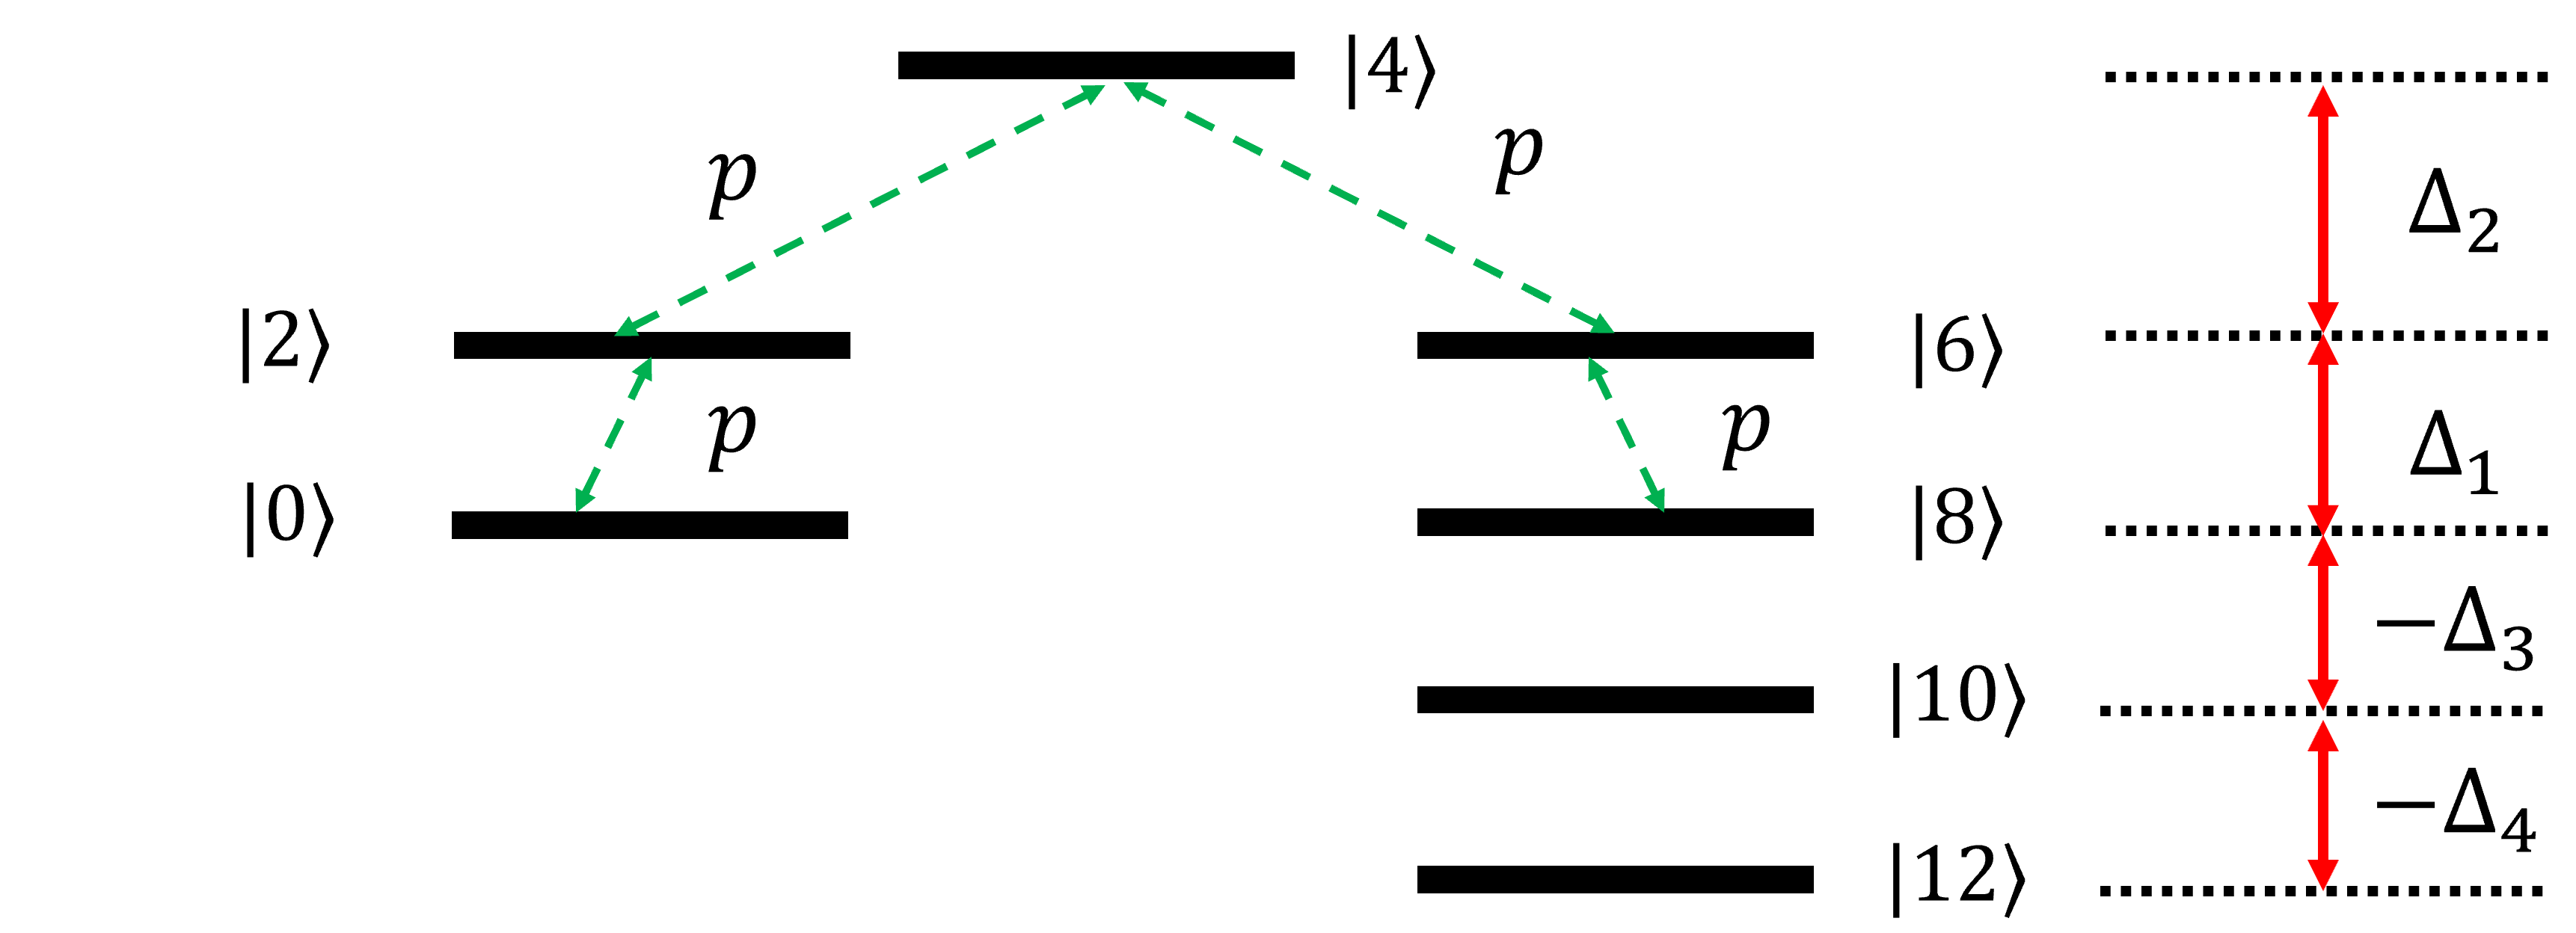
\includegraphics[width=10cm]{file/fig/effective_0and8/KPO_effective_0and8.png} \\
\caption{有効模型の概念図}
\label{fig:kpo_effective_0and8}
\end{figure}

\begin{align}
     \hat{H}_{\rm{KPO}}^{\rm{eff}}&=
   \bordermatrix{     
    & \bra{0} &  \bra{2} &  \bra{4}&  \bra{6}&  \bra{8} &\bra{10} &\bra{12}\cr
   \ket{0}&E_0&p_1&0&0&0&0&0\cr
  \ket{2}&p_1&E_2&p_2&0&0&0&0\cr
  \ket{4}&0&p_2&E_4&p_3&0&0&0\cr
  \ket{6}&0&0&p_3&E_6&p_4&0&0\cr
  \ket{8}&0&0&0&p_4&E_8&p_5&0\cr
  \ket{10}&0&0&0&0&p_5&E_{10}&p_6\cr
  \ket{12}&0&0&0&0&0&p_6&E_{12}\cr
            }
    %%%
    =
   \bordermatrix{     
    & \bra{0} &  \bra{2} &  \bra{4}&  \bra{6}&  \bra{8} &\bra{10} &\bra{12}\cr
   \ket{0}&0&p_1&0&0&0&0&0\cr
  \ket{2}&p_1&\Delta_1&p_2&0&0&0&0\cr
  \ket{4}&0&p_2&\Delta_2&p_3&0&0&0\cr
  \ket{6}&0&0&p_3&\Delta_1&p_4&0&0\cr
  \ket{8}&0&0&0&p_4&0&p_5&0\cr
  \ket{10}&0&0&0&0&p_5&-\Delta_3&p_6\cr
  \ket{12}&0&0&0&0&0&p_6&-\Delta_4\cr
            }\nn[10pt]
    %%%%%%%%%%%%%%%%%%%
    &=\hat{H}_0 + \hat{V} 
\end{align}
ここで,この有効模型の非摂動Hamiltonian $\hat{H}_0^{\rm{eff}}$と摂動Hamiltonian $\hat{V}^{\rm{eff}}$はそれぞれ以下のように与える:
\begin{align}
    \hat{H}_0^{\rm{eff}}&=\bordermatrix{
    & \bra{0} &  \bra{2} &  \bra{4}&  \bra{6}&  \bra{8} &\bra{10} &\bra{12}\cr
   \ket{0}&0&p&0&0&0&0&0\cr
  \ket{2}&p&\Delta_1&p&0&0&0&0\cr
  \ket{4}&0&p&\Delta_2&p&0&0&0\cr
  \ket{6}&0&0&p&\Delta_1&p&0&0\cr
  \ket{8}&0&0&0&p&0&0&0\cr
  \ket{10}&0&0&0&0&0&-\Delta_3&0\cr
  \ket{12}&0&0&0&0&0&0&-\Delta_4\cr}\nn[10pt]
  %%%%%%%%%%%%%%
  %%%%%%%%%%%%%%
  \hat{V}^{\rm{eff}}&=
   \bordermatrix{     
    & \bra{0} &  \bra{2} &  \bra{4}&  \bra{6}&  \bra{8} &\bra{10} &\bra{12}\cr
   \ket{0}&0&p_1-p&0&0&0&0&0\cr
  \ket{2}&p_1-p&0&p_2-p&0&0&0&0\cr
  \ket{4}&0&p_2-p&0&p_3-p&0&0&0\cr
  \ket{6}&0&0&p_3-p&0&p_4-p&0&0\cr
  \ket{8}&0&0&0&p_4-p&0&p_5&0\cr
  \ket{10}&0&0&0&0&p_5&0&p_6\cr
  \ket{12}&0&0&0&0&0&p_6&0\cr}\\[10pt]
    &=
   \bordermatrix{     
    & \bra{0} &  \bra{2} &  \bra{4}&  \bra{6}&  \bra{8} &\bra{10} &\bra{12}\cr
   \ket{0}&0&\sqrt{2\cdot1}p&0&0&0&0&0\cr
  \ket{2}&\sqrt{2\cdot1}p&0&\sqrt{4\cdot3}p&0&0&0&0\cr
  \ket{4}&0&\sqrt{4\cdot3}p&0&\sqrt{6\cdot5}p&0&0&0\cr
  \ket{6}&0&0&\sqrt{6\cdot5}p&0&\sqrt{8\cdot7}p&0&0\cr
  \ket{8}&0&0&0&\sqrt{8\cdot7}p&0&\sqrt{10\cdot9}p&0\cr
  \ket{10}&0&0&0&0&\sqrt{10\cdot9}p&0&\sqrt{12\cdot11}p\cr
  \ket{12}&0&0&0&0&0&\sqrt{12\cdot11}p&0\cr
            }
\end{align}
ここで,$p_1=\sqrt{2\cdot1}p$, $p_2=\sqrt{4\cdot3}p$, $p_3=\sqrt{6\cdot5}p$, $p_4=\sqrt{8\cdot7}p$, $p_5=\sqrt{10\cdot9}p$, $p_6=\sqrt{12\cdot11}p$である.


\subsection{}
\begin{figure}[h]
\centering
		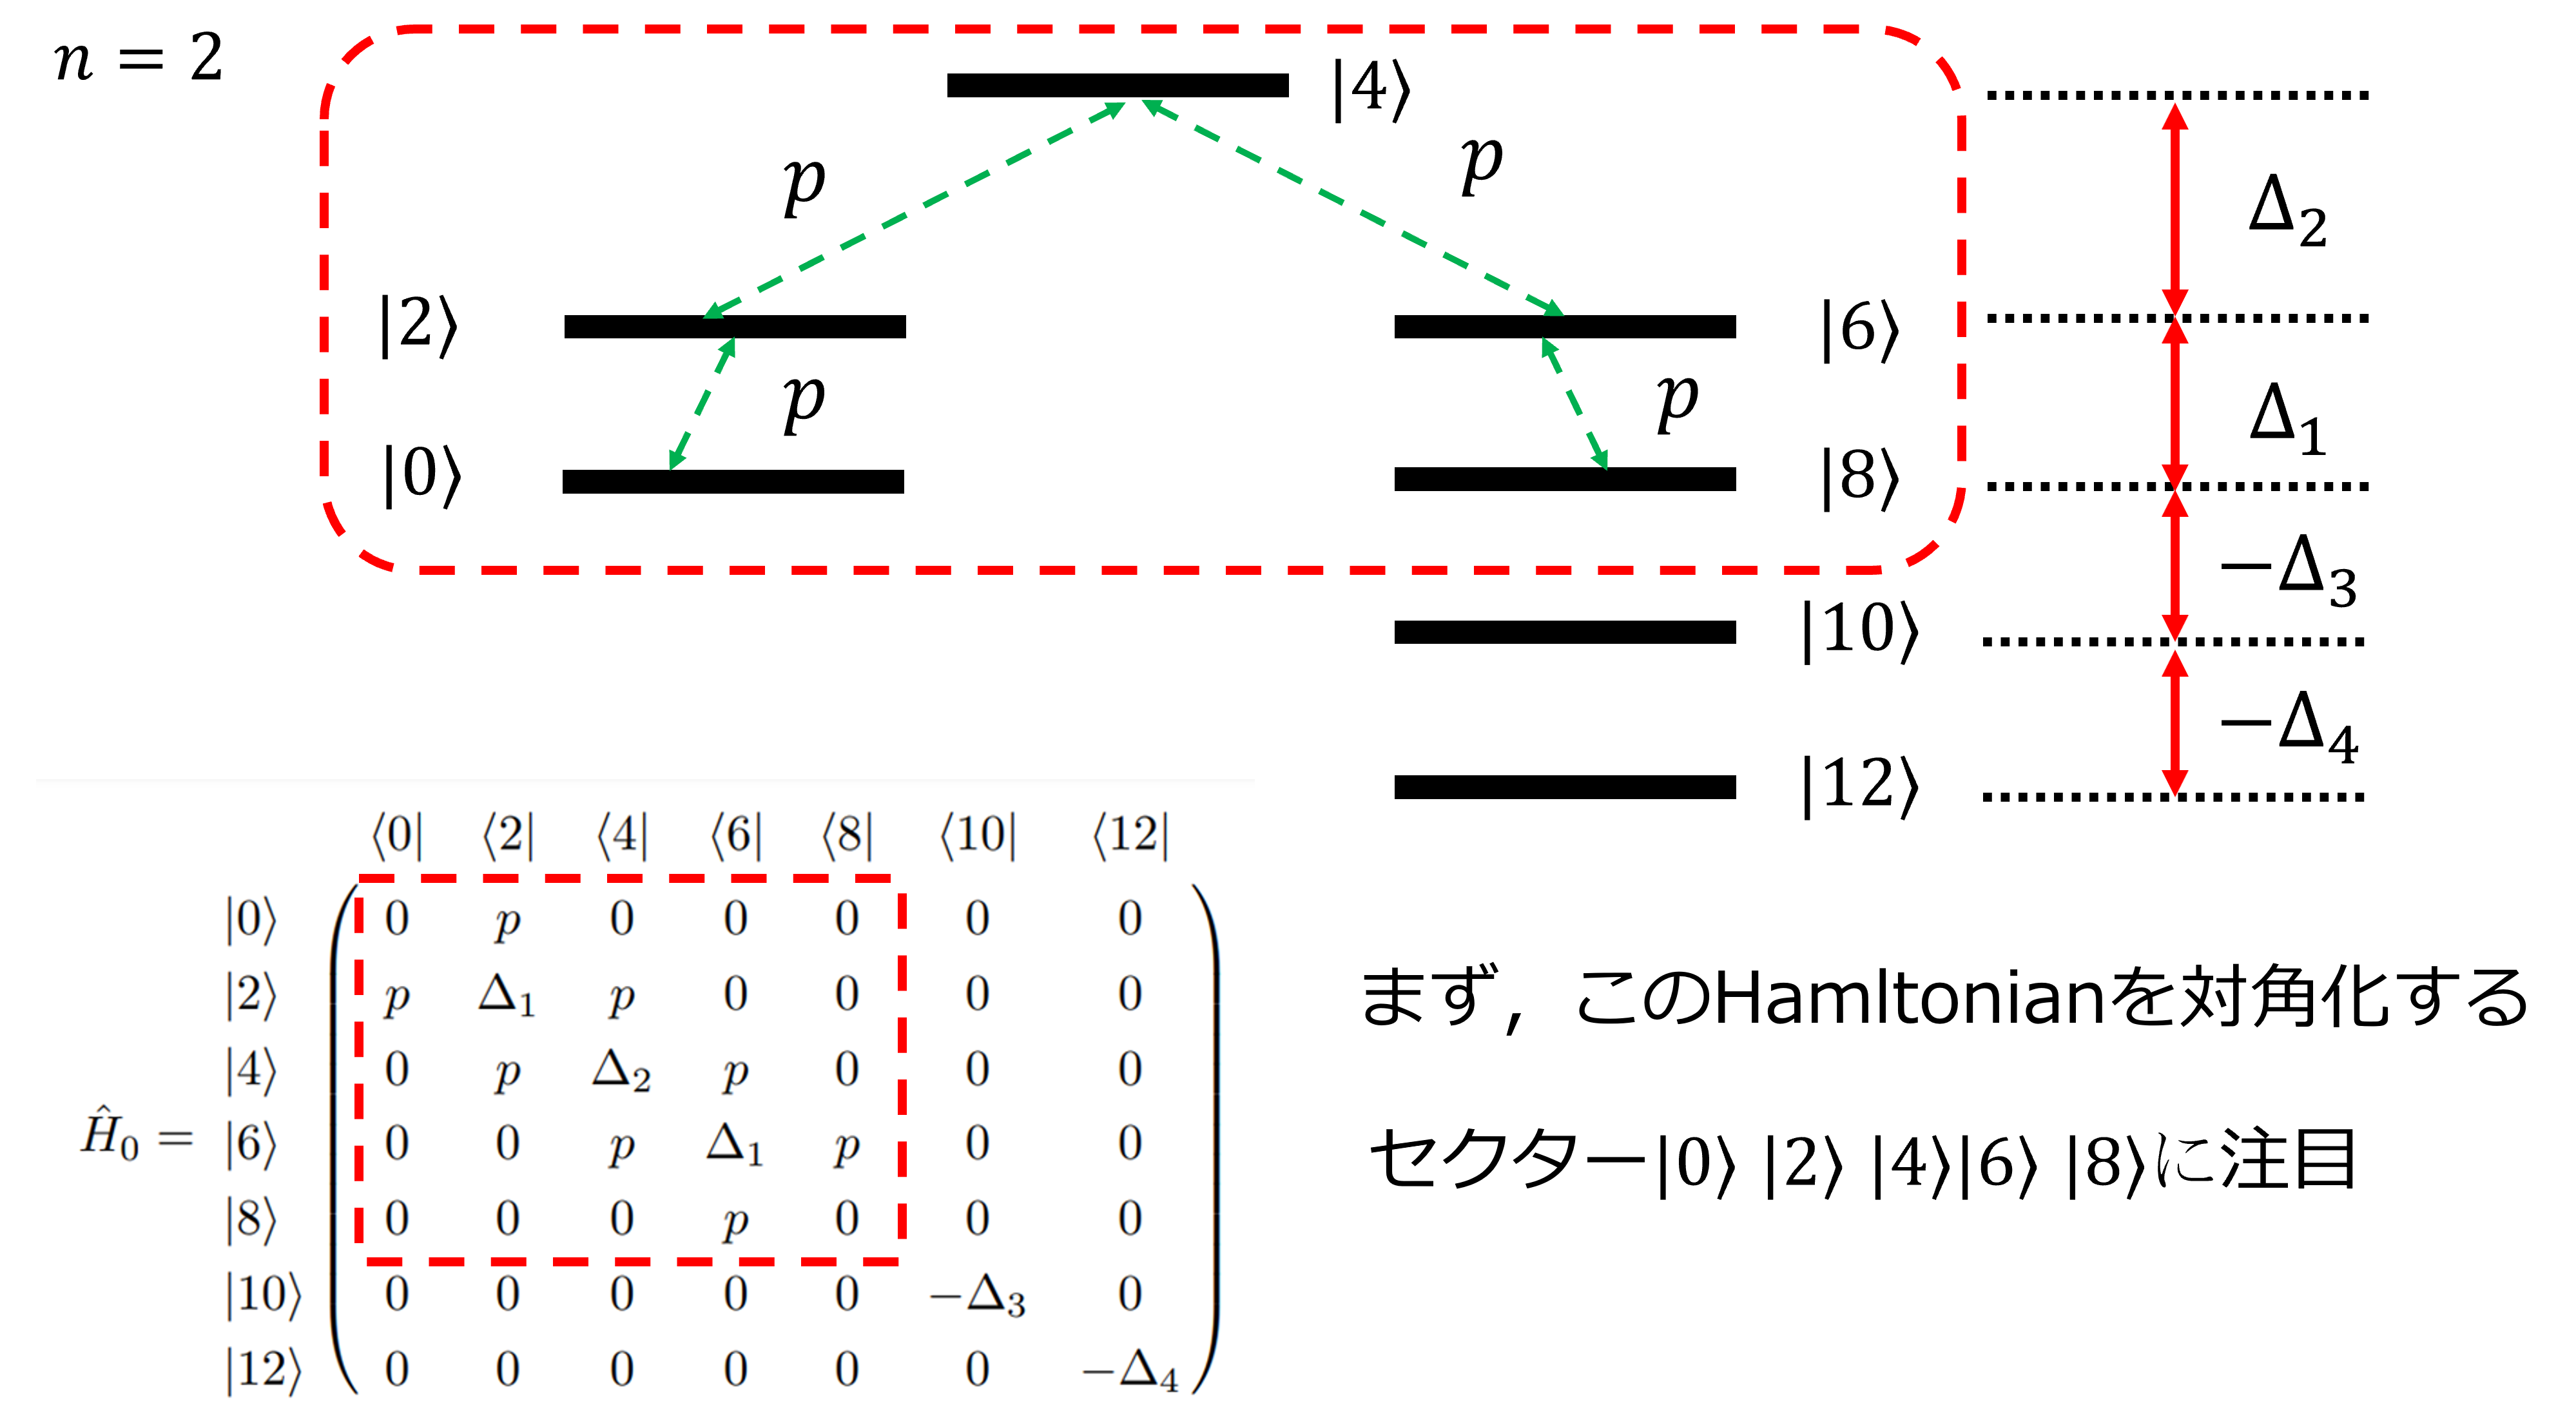
\includegraphics[width=10cm]{file/fig/effective_0and8/KPO_effective_0and8_1.png} \\
\caption{有効模型の概念図}
\label{fig:kpo_effective_0and8_1}
\end{figure}
次に,この有効模型の非摂動Hamiltonian $\hat{H}_0^{\rm{eff}}$に注目する.このHamiltonian $\hat{H}_0^{\rm{eff}}$はBlock対角化されており,$\{\ket{0}, \ket{2}, \ket{4}, \ket{6}, \ket{8}\}$と$\ket{10}, \ket{12}$で張られる部分空間に分けることができ, Hamiltonianは以下のように書き直すことができる:
\begin{equation}
    \hat{H}_0^{\rm{eff}}
    =\hat{H}_0^{0\to8} \bigoplus \hat{H}_0^{10,12}
\end{equation}
ここで,
    
\begin{align}
    \hat{H}_0^{0\to8}&=\bordermatrix{
    & \bra{0} &  \bra{2} &  \bra{4}&  \bra{6}&  \bra{8}\cr
   \ket{0}&0&p&0&0&0\cr
  \ket{2}&p&\Delta_1&p&0&0\cr
  \ket{4}&0&p&\Delta_2&p&0\cr
  \ket{6}&0&0&p&\Delta_1&p\cr
  \ket{8}&0&0&0&p&0\cr
  }\\[10pt]
  %%%%%%%%%%%%%%
  %%%%%%%%%%%%%%
  \hat{H}_0^{10,12}&=
   \bordermatrix{     
    & \bra{10} &\bra{12}\cr
   \ket{10}&-\Delta_3&0\cr
  \ket{12}&0&-\Delta_4\cr}
\end{align}
である.Hamiltonian $\hat{H}_0^{0\to8}$を対角化する.

これを実行するために,まず,$\{\ket{2}, \ket{4}, \ket{6}\}$で張られる部分空間を考え,その空間におけるHamiltonian $\hat{H}^{2,4,6}$を以下のように定義する:
\begin{align}
    \hat{H}^{2,4,6}&=\bordermatrix{
    & \bra{2} &  \bra{4}&  \bra{6}\cr
  \ket{2}&\Delta_1&p&0\cr
  \ket{4}&p&\Delta_2&p\cr
  \ket{6}&0&p&\Delta_1\cr
  }
\end{align}
\begin{figure}[h]
\centering
		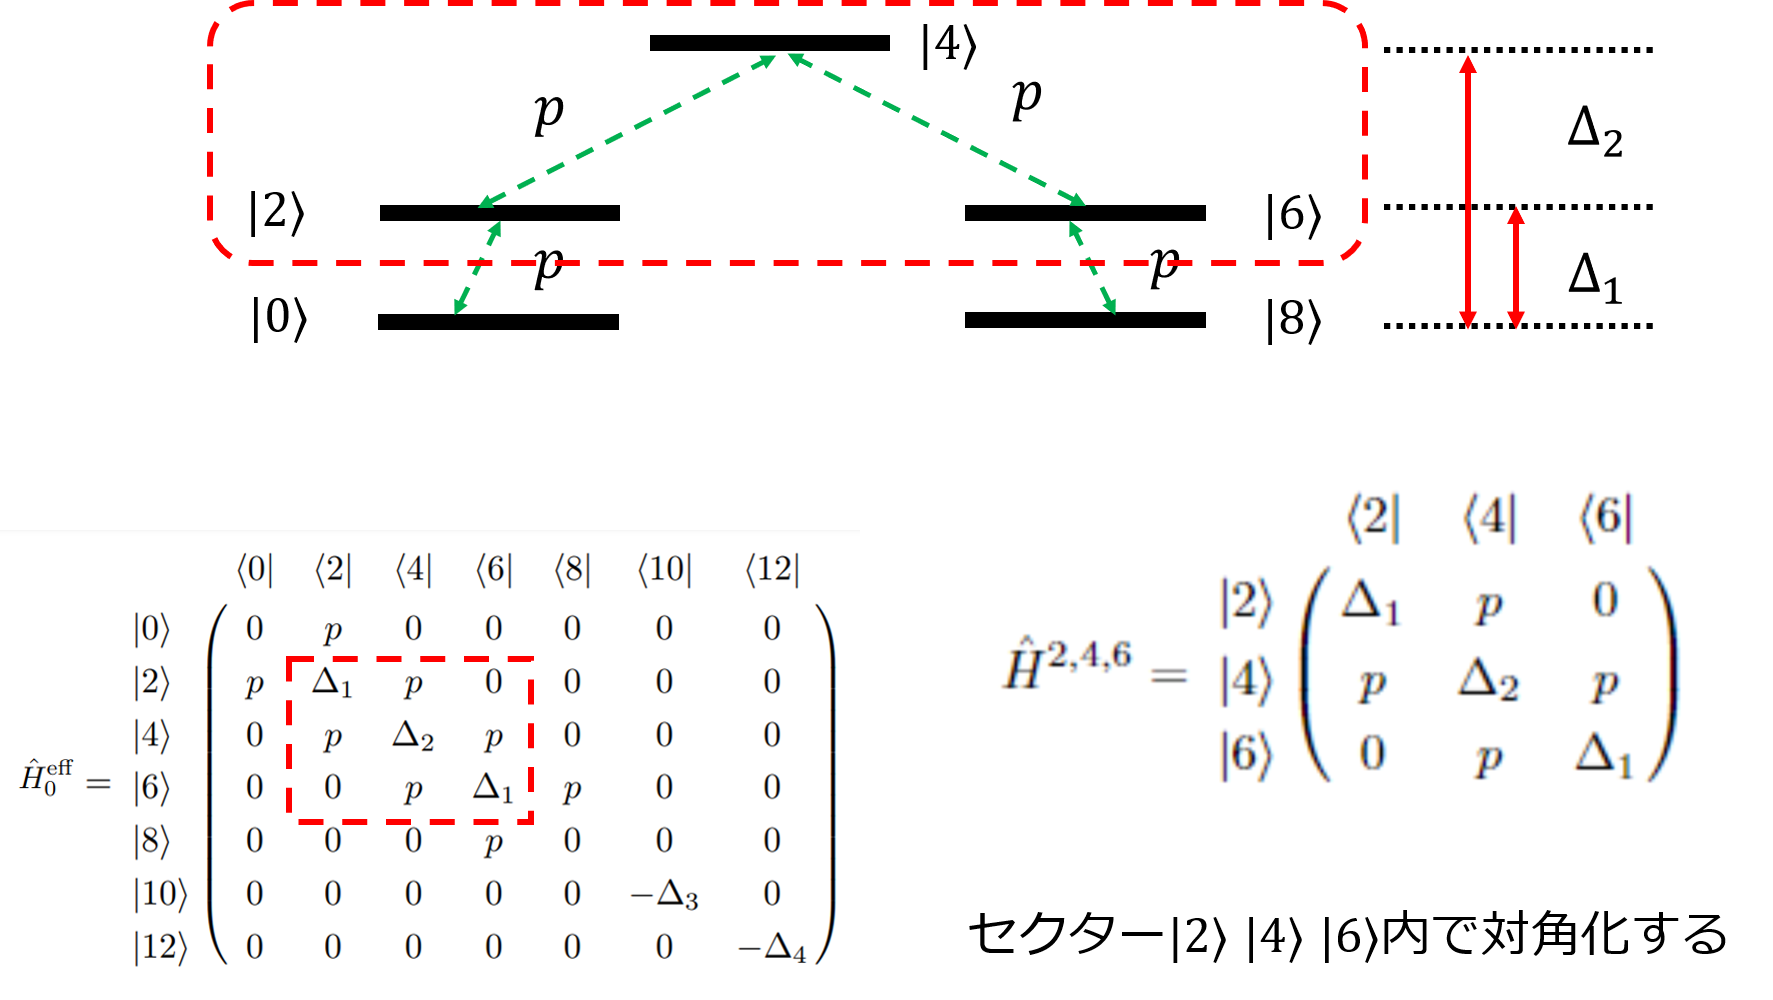
\includegraphics[width=10cm]{file/fig/effective_0and8/KPO_effective_0and8_3.png} \\
\caption{有効模型の概念図}
\label{fig:kpo_effective_0and8_3}
\end{figure}
ここで,$\Delta_1>\Delta_2$を仮定する.このHamiltonianを対角化し,エネルギー固有値とエネルギー固有状態を求めると以下のように得られる:
% \begin{align}
%     \left(\begin{array}{ccc}
%   \Delta_1&p&0\\[5pt]
%   p&\Delta_2&p\\[5pt]
%   0&p&\Delta_1\\[5pt]
%   \end{array}\right)    
% \end{align}
\begin{align}
    E_{D_{2,6}}&=
    {\Delta_{1}}\\[10pt]
    %
    E_{B_{2,6}}&=
    \frac{1}{2}\left(\Delta_1+\Delta_2-\sqrt{\Delta_1^2-2\Delta_1\Delta_2+\Delta_2^2+8p^2}\right)&\nn[10pt]
    &=\frac{1}{2}\left({\Delta_{1}}+{\Delta_{2}}-\sqrt{{
    (\Delta_{2}}-{\Delta_{1}})^2+8{p}^2}\right)\\[10pt]
    %%
    E_4=&\frac{1}{2}\left(\Delta_1+\Delta_2+\sqrt{\Delta_1^2-2\Delta_1\Delta_2+\Delta_2^2+8p^2}\right)
    \nn[10pt]
    &=\frac{1}{2}\left({\Delta_{1}}+{\Delta_{2}}
    +\sqrt{{
    (\Delta_{2}}-{\Delta_{1}})^2+8p^2}\right)
\end{align}
ここで,$E_{D_{2,6}} > E_{B_{2,6}} > E_4$である.固有状態は$\ket{2}, \ket{4}, \ket{6}$の基底で展開すれば以下のように得られる:
\begin{align}
    \ket{\psi_D}&=C_0\left\{-1,0,1\right\}\\[10pt]
    \ket{\psi_B}&=C_1\left\{1,-\frac{\Delta_1-\Delta_2+\sqrt{\Delta_1^2-2\Delta_1\Delta_2+\Delta_2^2+8p^2}}{2p},1\right\}\nn[10pt]
    &=C_1\left\{1,-\frac{{\Delta_{1}}-{\Delta_{2}}
    +\sqrt{({\Delta_{1}}-{\Delta_{2}})^2+8{p^2}}}{2{p}},1\right\}\nn[10pt]
    &=C_1\left\{1,
    \epsilon_+({\Delta_{1}},{\Delta_{2}},
    p)
    ,1\right\}\\[10pt]
    %
    %
    \ket{\psi_4}&=C_2\left\{1,-\frac{\Delta_1-\Delta_2-\sqrt{\Delta_1^2-2\Delta_1\Delta_2+\Delta_2^2+8p^2}}{2p},1\right\}\nn[10pt]
    &=C_2\left\{1,
    \epsilon_-({\Delta_{1}},{\Delta_{2}},
    p)
    ,1\right\}
\end{align}

\begin{align}
    \epsilon_{\textcolor{red}{\pm}}
    ({\Delta_{1}},{\Delta_{2}}, p)
    =-\frac{
    \Delta_{1}-\Delta_{2}
    {\textcolor{red}{\pm}}
    \sqrt{({\Delta_{1}}-{\Delta_{2}})^2+8{p^2}}
    }
    {2p}
\end{align}
規格化すると,
\begin{equation}
        \ket{D}\equiv\ket{\psi_0}=\left(
        \begin{array}{c}
       -\frac{1}{\sqrt{2}}\\[20pt]
       0\\[10pt]
       \frac{1}{\sqrt{2}}\\[10pt]
        \end{array}
        \right)
\end{equation}

\begin{equation}
     \ket{4}\equiv\ket{\psi_1}=\left(
        \begin{array}{c}
       \frac{1}{\sqrt{
       |\epsilon_{+}|^2
       +2}}\\[20pt]
       %
       %
       -\frac{{\Delta_1}-{\Delta_2}+\sqrt{{\Delta_1}^2-2{\Delta_1}{\Delta_2}+{\Delta_2}^2+8p^2}}{2{p_2}\sqrt{
       |\epsilon_{+}|^2+2}}\\[20pt]
       %
       %
       \frac{1}{\sqrt{
       |\epsilon_{+}|^2+2}}
        \end{array}
        \right)
        %%%%%%%%%%%%%%%%%%%%%%%%%%%%
        %%%%%%%%%%%%%%%%%%%%%%%%%%%%
        =\left(
        \begin{array}{c}
       \frac{1}{\sqrt{
       |\epsilon_{+}|^2
       +2}}\\[20pt]
       %
       %
       \frac{\epsilon_+}{
       \sqrt{
       |\epsilon_{+}|^2
       +2}}\\[20pt]
       %
       %
       \frac{1}{\sqrt{
       |\epsilon_{+}|^2
       +2}}
        \end{array}
        \right)
\end{equation}

\begin{equation}
     \ket{B}\equiv\ket{\psi_2}=\left(
        \begin{array}{c}
       \frac{1}{\sqrt{
       |\epsilon_{-}|^2
       +2}}\\[20pt]
       %
       %
       -\frac{{\Delta_1}-{\Delta_2}-\sqrt{{\Delta_1}^2-2{\Delta_1}{\Delta_2}+{\Delta_2}^2+8p^2}}{2{p_2}\sqrt{
       |\epsilon_{-}|^2
       +2}}\\[20pt]
       %
       %
       \frac{1}{\sqrt{
       |\epsilon_{-}|^2
       +2}}\\[10pt]
        \end{array}
        \right)
    %%%%%%%%%%%%%%%%%%%%%%%%%%%
    %%%%%%%%%%%%%%%%%%%%%%%%%%
    =\left(
        \begin{array}{c}
       \frac{1}{\sqrt{
       |\epsilon_{-}|^2
       +2}}\\[20pt]
       %
       %
       \frac{
       \epsilon_-
       }{\sqrt{
       |\epsilon_{-}|^2
       +2}}\\[20pt]
       %
       %
       \frac{1}{\sqrt{
       |\epsilon_{-}|^2
       +2}}\\[10pt]
        \end{array}
        \right)
\end{equation}
を得る.$\Delta_1 < \Delta_2$の場合は,$\ket{B}$と$\ket{4}$の正負が入れ替わることに注意.パラメトリックドライブの振幅が十分小さいことを仮定すれば,固有状態として,
\begin{align}
    \ket{D_{2,6}} &= \frac{1}{\sqrt{2}}(-\ket{2}+\ket{6})\\[10pt]
    \ket{B_{2,6}} &= \frac{1}{\sqrt{2}}(\ket{2}+\ket{6})
\end{align}
を定義できる.



\subsection{}
部分空間$\{\ket{2}, \ket{4}, \ket{6}\}$内で,対角化することができたため,これで,$\ket{2}$と$\ket{6}$の縮退を解くことができた.したがって,次に,Hamiltonian $\hat{H}_0^{0\to8}$に対して,縮退する摂動論を適用し,そのエネルギー固有値と対応するエネルギー固有状態を求めていくことにする.
\begin{figure}[h]
\centering
		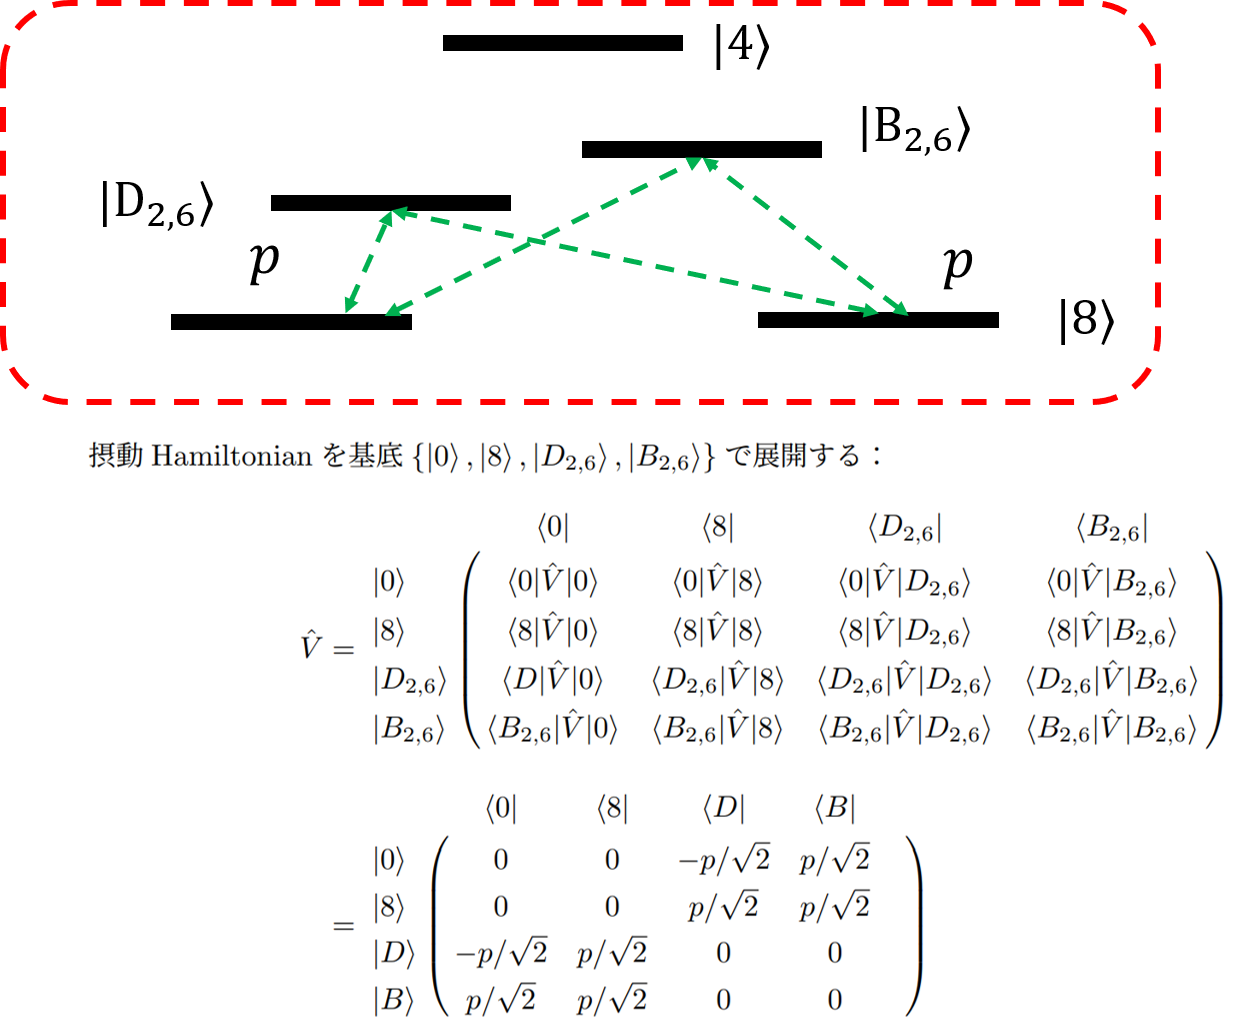
\includegraphics[width=10cm]{file/fig/effective_0and8/KPO_effective_0and8_4.png} \\
\caption{有効模型の概念図}
\label{fig:kpo_effective_0and8_4}
\end{figure}






% \subsection{縮退のない摂動論への移行}
% \begin{align}
%      \hat{H}_{\rm{KPO}}&=
%    \bordermatrix{     
%     & \bra{0} &  \bra{2} &  \bra{4}&  \bra{6}&  \bra{8} &\bra{10} &\bra{12}\cr
%    \ket{0}&E_0&p_1&0&0&0&0&0\cr
%   \ket{2}&p_1&E_2&p_2&0&0&0&0\cr
%   \ket{4}&0&p_2&E_4&p_3&0&0&0\cr
%   \ket{6}&0&0&p_3&E_6&p_4&0&0\cr
%   \ket{8}&0&0&0&p_4&E_8&p_5&0\cr
%   \ket{10}&0&0&0&0&p_5&E_{10}&p_6\cr
%   \ket{12}&0&0&0&0&0&p_6&E_{12}\cr
%             }
%     %%%
%     =
%    \bordermatrix{     
%     & \bra{0} &  \bra{2} &  \bra{4}&  \bra{6}&  \bra{8} &\bra{10} &\bra{12}\cr
%    \ket{0}&0&p_1&0&0&0&0&0\cr
%   \ket{2}&p_1&\Delta_1&p_2&0&0&0&0\cr
%   \ket{4}&0&p_2&\Delta_2&p_3&0&0&0\cr
%   \ket{6}&0&0&p_3&\Delta_1&p_4&0&0\cr
%   \ket{8}&0&0&0&p_4&0&p_5&0\cr
%   \ket{10}&0&0&0&0&p_5&-\Delta_3&p_6\cr
%   \ket{12}&0&0&0&0&0&p_6&-\Delta_4\cr
%             }\nn[10pt]
%     %%%%%%%%%%%%%%%%%%%
%     &=\hat{H}_0 + \hat{V} 
% \end{align}


% \begin{align}
%     \hat{H}_0&=\bordermatrix{
%     & \bra{0} &  \bra{2} &  \bra{4}&  \bra{6}&  \bra{8} &\bra{10} &\bra{12}\cr
%    \ket{0}&0&p&0&0&0&0&0\cr
%   \ket{2}&p&\Delta_1&p&0&0&0&0\cr
%   \ket{4}&0&p&\Delta_2&p&0&0&0\cr
%   \ket{6}&0&0&p&\Delta_1&p&0&0\cr
%   \ket{8}&0&0&0&p&0&0&0\cr
%   \ket{10}&0&0&0&0&0&-\Delta_3&0\cr
%   \ket{12}&0&0&0&0&0&0&-\Delta_4\cr}\nn[10pt]
%   %%%%%%%%%%%%%%
%   %%%%%%%%%%%%%%
%   \hat{V}&=
%    \bordermatrix{     
%     & \bra{0} &  \bra{2} &  \bra{4}&  \bra{6}&  \bra{8} &\bra{10} &\bra{12}\cr
%    \ket{0}&0&p_1-p&0&0&0&0&0\cr
%   \ket{2}&p_1-p&0&p_2-p&0&0&0&0\cr
%   \ket{4}&0&p_2-p&0&p_3-p&0&0&0\cr
%   \ket{6}&0&0&p_3-p&0&p_4-p&0&0\cr
%   \ket{8}&0&0&0&p_4-p&0&p_5&0\cr
%   \ket{10}&0&0&0&0&p_5&0&p_6\cr
%   \ket{12}&0&0&0&0&0&p_6&0\cr}\\[10pt]
%     &=
%    \bordermatrix{     
%     & \bra{0} &  \bra{2} &  \bra{4}&  \bra{6}&  \bra{8} &\bra{10} &\bra{12}\cr
%    \ket{0}&0&\sqrt{2\cdot1}p&0&0&0&0&0\cr
%   \ket{2}&\sqrt{2\cdot1}p&0&\sqrt{4\cdot3}p&0&0&0&0\cr
%   \ket{4}&0&\sqrt{4\cdot3}p&0&\sqrt{6\cdot5}p&0&0&0\cr
%   \ket{6}&0&0&\sqrt{6\cdot5}p&0&\sqrt{8\cdot7}p&0&0\cr
%   \ket{8}&0&0&0&\sqrt{8\cdot7}p&0&\sqrt{10\cdot9}p&0\cr
%   \ket{10}&0&0&0&0&\sqrt{10\cdot9}p&0&\sqrt{12\cdot11}p\cr
%   \ket{12}&0&0&0&0&0&\sqrt{12\cdot11}p&0\cr
%             }
% \end{align}
% $p_1=\sqrt{2\cdot1}p$, $p_2=\sqrt{4\cdot3}p$, $p_3=\sqrt{6\cdot5}p$, $p_4=\sqrt{8\cdot7}p$, $p_5=\sqrt{10\cdot9}p$, $p_6=\sqrt{12\cdot11}p$
  
%%%%%%%%%%%%%%%%%%%%%%%%%%%%%%%%%%%%%
% \subsection{部分空間での計算}
% 次の状態を定義する:
% \begin{align}
%     \ket{D_{2,6}} &= \frac{1}{\sqrt{2}}(-\ket{2}+\ket{6})\\[10pt]
%     \ket{B_{2,6}} &= \frac{1}{\sqrt{2}}(\ket{2}+\ket{6})
% \end{align}
そのために,まず,摂動Hamiltonianを基底$\{\ket{0},\ket{8},\ket{D_{2,6}},\ket{B_{2,6}}\}$で展開する:
\begin{align}
     \hat{V}
    &=
   \bordermatrix{     
    & \bra{0} &  \bra{8} &  \bra{D_{2,6}}&  \bra{B_{2,6}}\cr
   \ket{0}&\langle{0|\hat{V}|0}\rangle&\langle{0|\hat{V}|8}\rangle&\langle{0|\hat{V}|D_{2,6}}\rangle
   &\langle{0|\hat{V}|B_{2,6}}\rangle\cr
  \ket{8}&\langle{8|\hat{V}|0}\rangle&\langle{8|\hat{V}|8}\rangle&\langle{8|\hat{V}|D_{2,6}}\rangle
   &\langle{8|\hat{V}|B_{2,6}}\rangle\cr
  \ket{D_{2,6}}&\langle{D|\hat{V}|0}\rangle&\langle{D_{2,6}|\hat{V}|8}\rangle&\langle{D_{2,6}|\hat{V}|D_{2,6}}\rangle
   &\langle{D_{2,6}|\hat{V}|B_{2,6}}\rangle\cr
  \ket{B_{2,6}}&\langle{B_{2,6}|\hat{V}|0}\rangle&\langle{B_{2,6}|\hat{V}|8}\rangle&\langle{B_{2,6}|\hat{V}|D_{2,6}}\rangle
   &\langle{B_{2,6}|\hat{V}|B_{2,6}}\rangle\cr
    }\\[10pt]
    &=
   \bordermatrix{     
    & \bra{0} &  \bra{8} &  \bra{D}&  \bra{B}\cr
   \ket{0}&0&0&-p/\sqrt{2}&p/\sqrt{2}\cr
  \ket{8}&0&0&p/\sqrt{2}&p/\sqrt{2}\cr
  \ket{D}&-p/\sqrt{2}&p/\sqrt{2}&0&0\cr
  \ket{B}&p/\sqrt{2}&p/\sqrt{2}&0&0&\cr
            }
\end{align}

\begin{align}
    \langle{0|\hat{V}|D}\rangle&=\langle{D|\hat{V}|0}\rangle=-p/\sqrt{2}\\[10pt]
    \langle{0|\hat{V}|B}\rangle&=\langle{B|\hat{V}|0}\rangle=p/\sqrt{2}\\[10pt]
    \langle{8|\hat{V}|D}\rangle&=\langle{D|\hat{V}|8}\rangle=p/\sqrt{2}\\[10pt]
   \langle{8|\hat{V}|B}\rangle&=\langle{B|\hat{V}|8}\rangle=p/\sqrt{2}
\end{align}

\section*{\textcolor{red}{STEP1 : 固有状態の1次摂動を計算する}}
この摂動Hamiltonianに従って,摂動論を適用していく.まず,固有状態の1次摂動を計算する:
\begin{align}
    \ket{\varphi_{n,0}^{(1)}}
    &=
    \sum_{\textcolor{red}{\gamma\neq0}}|\varphi^{(0)}_n;8\rangle\rangle
    \textcolor{red}{\frac{1}{(E^{(2)}_{n,0}-E^{(2)}_{n,8})}
    \sum_{m\neq n}\Biggl[\sum_{p\neq n}
    \frac{\langle\braket{\varphi^{(0)}_{n};\gamma|\hat{V}|\varphi^{(0)}_m}
    \langle{\varphi^{(0)}_{m}|\hat{V}|\varphi^{(0)}_p}\rangle
    \braket{\varphi^{(0)}_{p}|\hat{V}|\varphi^{(0)}_n;0}\rangle}
    {(\epsilon_n-\epsilon_m)(\epsilon_n-\epsilon_p)}}\nn[10pt]
    %
    &\hspace{100pt}
    \textcolor{red}{-E^{(1)}_n
    \frac{\langle\braket{\varphi^{(0)}_{n};\gamma|\hat{V}|\varphi^{(0)}_m}
    \braket{\varphi^{(0)}_{m}|\hat{V}|\varphi^{(0)}_n;0}\rangle}{(\epsilon_n-\epsilon_m)^2}
    \Biggr]}
    \nn[10pt]
    %
    &\hspace{200pt}+
    \sum_{m\neq n}\ket{\varphi^{(0)}_m}
    \textcolor{blue}{
    \frac{\braket{\varphi^{(0)}_{m}|\hat{V}|\varphi^{(0)}_n;0}\rangle}{(\epsilon_n-\epsilon_m)}}\nn[10pt]
    %%%%%%%%%%%%%%%%%%%%
    %%%%%%%%%%%%%%%%%%%%
    &=
    |\varphi^{(0)}_n;8\rangle\rangle
    \textcolor{red}{\frac{1}{(E^{(2)}_{n,0}-E^{(2)}_{n,8})}
    \sum_{m\neq n}\Biggl[\sum_{p\neq n}
    \frac{\langle\braket{\varphi^{(0)}_{n};8|\hat{V}|\varphi^{(0)}_m}
    \langle{\varphi^{(0)}_{m}|\hat{V}|\varphi^{(0)}_p}\rangle
    \braket{\varphi^{(0)}_{p}|\hat{V}|\varphi^{(0)}_n;0}\rangle}
    {(\epsilon_n-\epsilon_m)(\epsilon_n-\epsilon_p)}}\nn[10pt]
    %
    &\hspace{100pt}
    \textcolor{red}{-E^{(1)}_n
    \frac{\langle\braket{\varphi^{(0)}_{n};8|\hat{V}|\varphi^{(0)}_m}
    \braket{\varphi^{(0)}_{m}|\hat{V}|\varphi^{(0)}_n;0}\rangle}{(\epsilon_n-\epsilon_m)^2}
    \Biggr]}
    \nn[10pt]
    %
    &\hspace{200pt}+
    \sum_{m\neq n}\ket{\varphi^{(0)}_m}
    \textcolor{blue}{
    \frac{\braket{\varphi^{(0)}_{m}|\hat{V}|\varphi^{(0)}_n;0}\rangle}{(\epsilon_n-\epsilon_m)}}\nn[10pt]
    %%%%%%%%%%%%%%%%%%%%
    %%%%%%%%%%%%%%%%%%%%
    &=
    |\varphi^{(0)}_n;8\rangle\rangle
    \textcolor{red}{\frac{1}{(E^{(2)}_{n,0}-E^{(2)}_{n,8})}
    \sum_{m\neq n}\Biggl[
    \frac{\langle\braket{\varphi^{(0)}_{n};8|\hat{V}|\varphi^{(0)}_m}
    \langle{\varphi^{(0)}_{m}|\hat{V}|\varphi^{(0)}_D}\rangle
    \braket{\varphi^{(0)}_{D}|\hat{V}|\varphi^{(0)}_n;0}\rangle}
    {(\epsilon_n-\epsilon_m)(\epsilon_n-\epsilon_D)}}\nn[10pt]
    %
    &\hspace{100pt}
    +{\frac{\langle\braket{\varphi^{(0)}_{n};8|\hat{V}|\varphi^{(0)}_m}
    \langle{\varphi^{(0)}_{m}|\hat{V}|\varphi^{(0)}_B}\rangle
    \braket{B|\hat{V}|\varphi^{(0)}_n;0}\rangle}
    {(\epsilon_n-\epsilon_m)(\epsilon_n-\epsilon_B)}}\nn[10pt]
    &\hspace{100pt}
    \textcolor{red}{-E^{(1)}_n
    \frac{\langle\braket{\varphi^{(0)}_{n};8|\hat{V}|\varphi^{(0)}_m}
    \braket{\varphi^{(0)}_{m}|\hat{V}|\varphi^{(0)}_n;0}\rangle}{(\epsilon_n-\epsilon_m)^2}
    \Biggr]}
    \nn[10pt]
    %
    &\hspace{200pt}+
    \sum_{m\neq n}\ket{\varphi^{(0)}_m}
    \textcolor{blue}{
    \frac{\braket{\varphi^{(0)}_{m}|\hat{V}|\varphi^{(0)}_n;0}\rangle}{(\epsilon_n-\epsilon_m)}}
\end{align}



\begin{align}
    \ket{\varphi_{n,0}^{(1)}}
    &=
    |\varphi^{(0)}_n;8\rangle\rangle
    \textcolor{red}{\frac{1}{(E^{(2)}_{n,0}-E^{(2)}_{n,8})}}\nn[10pt]
    &\times
    \textcolor{red}{\Biggl[\Biggl\{
    \frac{\langle\braket{\varphi^{(0)}_{n};8|\hat{V}|\varphi^{(0)}_D}
    \langle{\varphi^{(0)}_{D}|\hat{V}|\varphi^{(0)}_D}\rangle
    \braket{\varphi^{(0)}_{D}|\hat{V}|\varphi^{(0)}_n;0}\rangle}
    {(\epsilon_n-\epsilon_D)(\epsilon_n-\epsilon_D)}}\nn[10pt]
    %
    &\hspace{100pt}
    +{\frac{\langle\braket{\varphi^{(0)}_{n};8|\hat{V}|\varphi^{(0)}_D}
    \langle{\varphi^{(0)}_{D}|\hat{V}|\varphi^{(0)}_B}\rangle
    \braket{\varphi^{(0)}_{B}|\hat{V}|\varphi^{(0)}_n;0}\rangle}
    {(\epsilon_n-\epsilon_D)(\epsilon_n-\epsilon_B)}}\nn[10pt]
    &\hspace{100pt}
    \textcolor{red}{-E^{(1)}_n
    \frac{\langle\braket{\varphi^{(0)}_{n};8|\hat{V}|\varphi^{(0)}_D}
    \braket{\varphi^{(0)}_{D}|\hat{V}|\varphi^{(0)}_n;0}\rangle}{(\epsilon_n-\epsilon_D)^2}
    \Biggr\}}
    \nn[10pt]
    %
    %
    &+\textcolor{red}{\Biggl\{
    \frac{\langle\braket{\varphi^{(0)}_{n};8|\hat{V}|\varphi^{(0)}_B}
    \langle{\varphi^{(0)}_{B}|\hat{V}|\varphi^{(0)}_D}\rangle
    \braket{\varphi^{(0)}_{D}|\hat{V}|\varphi^{(0)}_n;0}\rangle}
    {(\epsilon_n-\epsilon_B)(\epsilon_n-\epsilon_D)}}\nn[10pt]
    %
    &\hspace{100pt}
    +{\frac{\langle\braket{\varphi^{(0)}_{n};8|\hat{V}|\varphi^{(0)}_B}
    \langle{\varphi^{(0)}_{B}|\hat{V}|\varphi^{(0)}_B}\rangle
    \braket{\varphi^{(0)}_{B}|\hat{V}|\varphi^{(0)}_n;0}\rangle}
    {(\epsilon_n-\epsilon_B)(\epsilon_n-\epsilon_B)}}\nn[10pt]
    &\hspace{100pt}
    \textcolor{red}{-E^{(1)}_n
    \frac{\langle\braket{\varphi^{(0)}_{n};8|\hat{V}|\varphi^{(0)}_B}
    \braket{\varphi^{(0)}_{B}|\hat{V}|\varphi^{(0)}_n;0}\rangle}{(\epsilon_n-\epsilon_B)^2}
    \Biggr\}\Biggr]}
    \nn[10pt]
    %
    %
    &+
    \ket{\varphi^{(0)}_D}
    \textcolor{blue}{
    \frac{\braket{\varphi^{(0)}_{D}|\hat{V}|\varphi^{(0)}_n;0}\rangle}{(\epsilon_n-\epsilon_D)}}
    +
    \ket{\varphi^{(0)}_B}
    \textcolor{blue}{
    \frac{\braket{\varphi^{(0)}_{B}|\hat{V}|\varphi^{(0)}_n;0}\rangle}{(\epsilon_n-\epsilon_B)}}
\end{align}

$|\varphi^{(0)}_{n};0\rangle\rangle=C_{0,0}\ket{0}+C_{8,0}\ket{8}$, 
$|\varphi^{(0)}_{n};8\rangle\rangle=C_{0,8}\ket{0}+C_{8,8}\ket{8}$,  $|\varphi^{(0)}_{D}\rangle=\ket{D}$, $|\varphi^{(0)}_{B}\rangle=\ket{B}$であるから,


\begin{align}
    \ket{\varphi_{n,0}^{(1)}}
    &=
    |\varphi^{(0)}_n;8\rangle\rangle
    \textcolor{red}{\frac{1}{(E^{(2)}_{n,0}-E^{(2)}_{n,8})}}\nn[10pt]
    &\times
    \textcolor{red}{\Biggl[\Biggl\{
    \frac{\langle\braket{\varphi^{(0)}_{n};8|\hat{V}|D}
    \langle{D|\hat{V}|D}\rangle
    \braket{D|\hat{V}|\varphi^{(0)}_n;0}\rangle}
    {(\epsilon_n-\epsilon_D)(\epsilon_n-\epsilon_D)}}\nn[10pt]
    %
    &\hspace{100pt}
    +{\frac{\langle\braket{\varphi^{(0)}_{n};8|\hat{V}|D}
    \langle{D|\hat{V}|B}\rangle
    \braket{B|\hat{V}|\varphi^{(0)}_n;0}\rangle}
    {(\epsilon_n-\epsilon_D)(\epsilon_n-\epsilon_B)}}\nn[10pt]
    &\hspace{100pt}
    \textcolor{red}{-E^{(1)}_n
    \frac{\langle\braket{\varphi^{(0)}_{n};8|\hat{V}|D}
    \braket{D|\hat{V}|\varphi^{(0)}_n;0}\rangle}{(\epsilon_n-\epsilon_D)^2}
    \Biggr\}}
    \nn[10pt]
    %
    %
    &+\textcolor{red}{\Biggl\{
    \frac{\langle\braket{\varphi^{(0)}_{n};8|\hat{V}|B}
    \langle{B|\hat{V}|D}\rangle
    \braket{D|\hat{V}|\varphi^{(0)}_n;0}\rangle}
    {(\epsilon_n-\epsilon_B)(\epsilon_n-\epsilon_D)}}\nn[10pt]
    %
    &\hspace{100pt}
    +{\frac{\langle\braket{\varphi^{(0)}_{n};8|\hat{V}|B}
    \langle{B|\hat{V}|B}\rangle
    \braket{B|\hat{V}|\varphi^{(0)}_n;0}\rangle}
    {(\epsilon_n-\epsilon_B)(\epsilon_n-\epsilon_B)}}\nn[10pt]
    &\hspace{100pt}
    \textcolor{red}{-E^{(1)}_n
    \frac{\langle\braket{\varphi^{(0)}_{n};8|\hat{V}|B}
    \braket{B|\hat{V}|\varphi^{(0)}_n;0}\rangle}{(\epsilon_n-\epsilon_B)^2}
    \Biggr\}\Biggr]}
    \nn[10pt]
    %
    %
    &+
    \ket{D}
    \textcolor{blue}{
    \frac{\braket{D|\hat{V}|\varphi^{(0)}_n;0}\rangle}{(\epsilon_n-\epsilon_D)}}
    +
    \ket{B}
    \textcolor{blue}{
    \frac{\braket{B|\hat{V}|\varphi^{(0)}_n;0}\rangle}{(\epsilon_n-\epsilon_B)}}
\end{align}

ここで,
\begin{equation}
    \langle{D|\hat{V}|D}\rangle
    =\langle{B|\hat{V}|B}\rangle
    =\langle{D|\hat{V}|B}\rangle
    =\langle{B|\hat{V}|D}\rangle=0
\end{equation}

\begin{equation}
    E^{(1)}_n = 0
\end{equation}

\begin{align}
    \braket{D|\hat{V}|\varphi^{(0)}_n;0}\rangle
    &=C_{0,0}\braket{D|\hat{V}|0} + C_{8,0}\braket{D|\hat{V}|8}
    =C_{0,0}(-p/\sqrt{2}) + C_{8,0} (p/\sqrt{2})\\[10pt]
    \braket{B|\hat{V}|\varphi^{(0)}_n;0}\rangle
    &=C_{0,0}\braket{B|\hat{V}|0} + C_{8,0}\braket{B|\hat{V}|8}
    =C_{0,0}(p/\sqrt{2}) + C_{8,0} (p/\sqrt{2})
\end{align}

であるから,

\begin{align}
    \ket{\varphi_{n,0}^{(1)}}
    &=
    \ket{D}
    \textcolor{blue}{
    \frac{\braket{D|\hat{V}|\varphi^{(0)}_n;0}\rangle}{(\epsilon_{0}-\epsilon_D)}}
    +
    \ket{B}
    \textcolor{blue}{
    \frac{\braket{B|\hat{V}|\varphi^{(0)}_n;0}\rangle}{(\epsilon_0-\epsilon_B)}}\\[10pt]
    &=\ket{D}
    \frac{1}{(\epsilon_{0}-\epsilon_D)}
    \Bigl\{C_{0,0}(-p/\sqrt{2}) + C_{8,0} (p/\sqrt{2})\Bigr\}\nn[10pt]
    &+
    \ket{B}
    \frac{1}{(\epsilon_{0}-\epsilon_B)}
    \Bigl\{C_{0,0}(p/\sqrt{2}) + C_{8,0} (p/\sqrt{2})\Bigr\}
\end{align}






\section*{\textcolor{red}{永年方程式を解き,2次の補正項と規格化定数を求める}}
永年方程式
\begin{align}\label{2ndpertubation_matrix}
\sum_{\beta=1}^{N}\Biggl[
E^{(2)}_n \delta_{\alpha,\beta}
-(\hat{V}^{(2)})_{\alpha,\beta}
\biggr]C_{\beta,\alpha}=0,
\end{align}
ここで,
\begin{equation}
    (\hat{V}^{(2)})_{\alpha,\beta}
    \equiv\sum_{m\neq n}
    \frac{\langle{\varphi^{(0)}_n;\alpha|\hat{V}|\varphi^{(0)}_m}\rangle
    \langle{\varphi^{(0)}_{m}|\hat{V}|\varphi^{(0)}_n;\beta}\rangle}
    {(\epsilon_n-\epsilon_m)}
\end{equation}
を解き,エネルギー固有値の2次の補正項$E_{n,0}^{(2)}$, $E_{n,8}^{(2)}$と固有状態の第ゼロ近似に関する展開係数,$C_{0,0}$, $C_{8,0}$, $C_{0,8}$, $C_{8,8}$を求める.





% この$C_{\beta}$に関する斉1次連立方程式が0以外の解を持つためには,$C_{\beta}$の係数のつくる行列が0でなくてはならない.すなわち,固有値$E^{(2)}_{n}$は以下の特性方程式の解である:
% \begin{equation}\label{2nd_eigen_eq}
%     \det{(E^{(2)}_n \delta_{\alpha,\beta}
%     -(\hat{V}^{(2)})_{\alpha,\beta})}=0
% \end{equation}
% この固有値方程式は重解も含めて$N$個の解 : $E^{(2)}_{n,\alpha}$, $(\alpha=1,2,\ldots,N)$を持つ.そして,$N$個のそれぞれの解$E^{(2)}_{n,\alpha}$を行列方程式に代入し,規格化条件$\sum_{\beta}|C_{\beta}|=1$のもとで,\eqref{2ndpertubation_matrix}を解くことにより,それぞれの解$E^{(2)}_{n,\alpha}$に対する係数が決定する.その係数を改めて$C_{\beta,\alpha}$と書き,これに対応する固有ベクトルを
% \begin{equation}
%     |\varphi^{(0)}_{n};\alpha\rangle\rangle
%     =\sum_{\beta=1}^{N}
%     \ket{\varphi^{(0)}_{n};\beta}C_{\beta,\alpha}
% \end{equation}
% と書き直す.これで第0近似での固有状態を決めることができた.固有状態$|\varphi^{(0)}_{n};\alpha\rangle\rangle$を\eqref{pereq2-1_degenerate}の$|\varphi^{(0)}_{n}\rangle\rangle$へ代入すると,
% \begin{align}
% (\epsilon_n-\epsilon_n)\braket{\varphi^{(0)}_n;\gamma|\varphi^{(2)}_n;\alpha}
% &=\langle{\varphi^{(0)}_n;\gamma|\hat{V}|\varphi^{(1)}_n;\alpha}\rangle
% -E^{(1)}_n\langle{\varphi^{(0)}_n;\gamma|\varphi^{(1)}_n;\alpha}\rangle
% -E^{(2)}\langle{\varphi^{(0)}_n;\gamma|\varphi^{(0)}_n;\alpha}\rangle\rangle
% %
% \end{align}
まず,非摂動ハミルトニアンのエネルギー固有値のうち,縮退していない状態のエネルギー固有値は以下のように与えられる:
\begin{align}
    \epsilon_D&=
    {\Delta_{1}}\\[10pt]
    %
    \epsilon_B&=
    \frac{1}{2}\left({\Delta_{1}}+{\Delta_{2}}-\sqrt{{\Delta_{1}}^2-2{\Delta_{1}}{\Delta_{2}}+{\Delta_{2}}^2+8{p}^2}\right)\nn[10pt]
    &=\frac{1}{2}\left({\Delta_{1}}+{\Delta_{2}}-\sqrt{{
    (\Delta_{1}}-{\Delta_{2}})^2+8{p}^2}\right)\nn[10pt]
    &=\frac{1}{2}\left({\Delta_{1}}+{\Delta_{2}}-\epsilon\right)\nn[10pt]
\end{align}
ここで,
\begin{align}
    \epsilon&\equiv
    \sqrt{{
    (\Delta_{1}}-{\Delta_{2}})^2+8{p}^2}
    ={(\Delta_{1}}-{\Delta_{2}})
    \sqrt{1+\frac{8{p}^2}{(\Delta_{1}-\Delta_{2})^2}}
    ={(\Delta_{1}}-{\Delta_{2}})\sqrt{1+\delta_+},\\[10pt]
    \delta_+ &\equiv \frac{8{p}^2}{(\Delta_{1}-\Delta_{2})^2}
\end{align}
とおいた.
次のTaylor展開の公式を
\begin{equation}
    \sqrt{1+x}
    =1+\frac{x}{2}-\frac{x^2}{8}+\frac{x^3}{16}-\frac{5x^4}{128}+\frac{7x^5}{256}+O\left(x^6\right)
\end{equation}
使うと,
\begin{align}
    \epsilon
    &\simeq{(\Delta_{1}}-{\Delta_{2}})
    \sqrt{1+\delta_{+}}\nn[10pt]
    &={(\Delta_{1}}-{\Delta_{2}})
    \Bigl(1+\frac{1}{2}\delta_{+}\Bigr)
    ={(\Delta_{1}}-{\Delta_{2}})
    \Bigl(1+\frac{4p^2}{(\Delta_{1}-\Delta_{2})^2}\Bigr)\nn[10pt]
    &={(\Delta_{1}}-{\Delta_{2}})
    +\frac{4p^2}{(\Delta_{1}-\Delta_{2})}
\end{align}
となり,エネルギー固有値$\epsilon_B$は以下のようになる:
\begin{equation}
    \epsilon_B
    \simeq\frac{1}{2}\left({\Delta_{1}}
    +{\Delta_{2}}+{(\Delta_{1}}-{\Delta_{2}})
    +\frac{4p^2}{(\Delta_{1}-\Delta_{2})}\right)
    =\Delta_1 + \frac{2p^2}{(\Delta_{1}-\Delta_{2})}
    =\Delta_1 + \delta_0
\end{equation}
ここで,
\begin{equation}
    \delta_0 \equiv \frac{2p^2}{(\Delta_{1}-\Delta_{2})}
\end{equation}

まず,2次摂動に関する行列要素を計算する:
\begin{align}
    (\hat{V}^{(2)})_{0,0}
    &=\sum_{m\neq n}
    \frac{\langle{0|\hat{V}|\varphi^{(0)}_m}\rangle
    \langle{\varphi^{(0)}_{m}|\hat{V}|0}\rangle}
    {(\epsilon_0-\epsilon_m)}
    =
    \frac{\langle{0|\hat{V}|B}\rangle
    \langle{B|\hat{V}|0}\rangle}
    {(-\epsilon_B)}
    +\frac{\langle{0|\hat{V}|D}\rangle
    \langle{D|\hat{V}|0}\rangle}
    {(-\epsilon_D)}\nn[10pt]
    %
    &=\frac{|\langle{0|\hat{V}|B}\rangle|^2}
    {(-\epsilon_B)}
    +\frac{|\langle{0|\hat{V}|D}\rangle|^2}
    {(-\epsilon_D)}
    =\frac{1 / 2}
    {(-\epsilon_B)}
    +\frac{1 / 2}
    {(-\epsilon_D)}
\end{align}


\begin{align}
    (\hat{V}^{(2)})_{8,8}
    &=\sum_{m\neq n}
    \frac{\langle{8|\hat{V}|\varphi^{(8)}_m}\rangle
    \langle{\varphi^{(8)}_{m}|\hat{V}|8}\rangle}
    {(\epsilon_8-\epsilon_m)}
    =
    \frac{\langle{8|\hat{V}|B}\rangle
    \langle{B|\hat{V}|8}\rangle}
    {(-\epsilon_B)}
    +\frac{\langle{8|\hat{V}|D}\rangle
    \langle{D|\hat{V}|8}\rangle}
    {(-\epsilon_D)}\nn[10pt]
    %
    &=\frac{|\langle{8|\hat{V}|B}\rangle|^2}
    {(-\epsilon_B)}
    +\frac{|\langle{8|\hat{V}|D}\rangle|^2}
    {(-\epsilon_D)}
    =\frac{1 / 2}
    {(-\epsilon_B)}
    +\frac{1 / 2}
    {(-\epsilon_D)}
\end{align}




\begin{align}
    (\hat{V}^{(2)})_{0,8}
    &=(\hat{V}^{(2)})_{8,0}
    =\sum_{m\neq n}
    \frac{\langle{0|\hat{V}|\varphi^{(8)}_m}\rangle
    \langle{\varphi^{(0)}_{m}|\hat{V}|8}\rangle}
    {(\epsilon_0-\epsilon_m)}
    =
    \frac{\langle{0|\hat{V}|B}\rangle
    \langle{B|\hat{V}|8}\rangle}
    {(-\epsilon_B)}
    +\frac{\langle{8|\hat{V}|D}\rangle
    \langle{D|\hat{V}|0}\rangle}
    {(-\epsilon_D)}\nn[10pt]
    & =
    \frac{1/2}
    {(-\epsilon_B)}
    +\frac{-1/2}
    {(-\epsilon_D)}
\end{align}





$\epsilon_B = \Delta_1 + \delta_0$, $\epsilon_D=\Delta_1$であるから,
\begin{align}
    (\hat{V}^{(2)})_{0,0}
    &
    =\frac{1 / 2}
    {(-\epsilon_B)}
    +\frac{1 / 2}
    {(-\epsilon_D)}
    =\frac{1/2}
    {-\Delta_1 - \delta_0}
    +\frac{1/2}
    {-\Delta_1}\nn[10pt]
    &
    =\frac{1}{2}
    \left(
    \frac{-\Delta_1-\Delta_1 - \delta_0}{-\Delta_1(-\Delta_1 + \delta_0)}
    \right)
    =\frac{1}{2}
    \left(\frac{-2\Delta_1 - \delta_0}{-\Delta_1(-\Delta_1 - \delta_0)}
    \right)
\end{align}


\begin{align}
    (\hat{V}^{(2)})_{8,8}
    &
    =\frac{1 / 2}
    {(-\epsilon_B)}
    +\frac{1 / 2}
    {(-\epsilon_D)}
    =\frac{1 / 2}
    {-\Delta_1 - \delta_0}
    +\frac{1 / 2}
    {-\Delta_1}
    =\frac{1}{2}\frac{-2\Delta_1 - \delta_0}{-\Delta_1(-\Delta_1 - \delta_0)}
\end{align}




\begin{align}
    (\hat{V}^{(2)})_{0,8}
    & =
    \frac{1/2}
    {(-\epsilon_B)}
    +\frac{-1/2}
    {(-\epsilon_D)}
    =\frac{1}{2}
    \Bigl(
    \frac{1}
    {-\Delta_1 - \delta_0}
    -\frac{1}
    {-\Delta_1}
    \Bigr)
    \nn[10pt]
    %
    &=\frac{1}{2}
    \Bigl(
    \frac{\delta_0}
    {-\Delta_1(-\Delta_1 - \delta_0)}
    \Bigr)
    =\frac{\delta_0}{B}
\end{align}


\begin{equation}
    E^{(2)}_n=\frac{
    (\hat{V}^{(2)})_{0,0} + (\hat{V}^{(2)})_{8,8}
    \mp \sqrt{D}
    }{2},
\end{equation}

\begin{align}
    D&=[(\hat{V}^{(2)})_{0,0} - \hat{V}^{(2)})_{8,8}]^2 + 4(\hat{V}^{(2)})_{0,8})^2\nn[10pt]
    &=4\frac{1}{4}\Bigl(
    \frac{\delta_0}
    {-\Delta_1(-\Delta_1 - \delta_0)}
    \Bigr)^2
    =\frac{\delta_0^2}
    {\{-\Delta_1(-\Delta_1 + \delta_0)\}^2}
\end{align}

よって,
\begin{align}
    E^{(2)}_n&=\frac{
    \frac{-2\Delta_1 - \delta_0}{-\Delta_1(-\Delta_1 - \delta_0)}
    \mp 
    \frac{\delta_0}
    {\{-\Delta_1(-\Delta_1 - \delta_0)\}}
    }{2}
    =\frac{
    (-2\Delta_1 - \delta_0)
    \mp \delta_0
    }{2\{-\Delta_1(-\Delta_1 - \delta_0)\}}
    =\frac{A}{B}[1\mp\delta_0/A]
\end{align}
ここで,
\begin{align}
    A&\equiv (-2\Delta_1 + \delta_0)\\[10pt]
    B&\equiv 2\{-\Delta_1(-\Delta_1 + \delta_0)\}\\[10pt]
    \delta_0 &= \frac{2p^2}{(\Delta_{1}-\Delta_{2})}
\end{align}
とおいた.

$E_n^{(2)}=E_{n,0}^{(2)}$のとき,規格化定数の比は
\begin{equation}
    \frac{C_{0,0}}{C_{0,8}} 
    = \frac{(\hat{V}^{(2)})_{0,0} - E_{n,0}^{(2)}}{2(\hat{V}^{(2)})_{0,8} }
    =  \frac{(\hat{V}^{(2)})_{0,0} - (\hat{V}^{(2)})_{8,8} \pm \sqrt{D}}
    {2(\hat{V}^{(2)})_{0,8} }
\end{equation}
となるから,
\begin{align}
    \frac{C_{0,0}}{C_{0,8}} 
    &= \frac{(\hat{V}^{(2)})_{0,0} - E_{n,0}^{(2)}}{2(\hat{V}^{(2)})_{0,8}}
    =  \frac{(\hat{V}^{(2)})_{0,0} - (\hat{V}^{(2)})_{8,8} \pm \sqrt{D}}
    {2(\hat{V}^{(2)})_{0,8} }
\end{align}


これより,$C_{0,0}=C_{0,8}=1/\sqrt{2}$を得る.すなわち,第0近似は
\begin{equation}
    \ket{\varphi_{n,0}^{0}} = \frac{1}{\sqrt{2}}(\ket{0}+\ket{8})
\end{equation}

第1次近似は
\begin{equation}
    \ket{\varphi_{n,0}^{1}} = \ket{B}\frac{p}{\epsilon_0-\epsilon_{B}}
\end{equation}
と求まるから,
\begin{equation}
     \ket{\varphi_{n,0}} 
     = \frac{1}{\sqrt{2}}(\ket{0}+\ket{8}) + \ket{B}\frac{p}{\epsilon_0-\epsilon_{B}}
\end{equation}






\section*{第8励起状態について,同様に計算を行う}
第8励起状態については,
\begin{align}
    \ket{\varphi_{n,8}^{(1)}}
    &=
    \sum_{\textcolor{red}{\gamma\neq8}}|\varphi^{(0)}_n;0\rangle\rangle
    \textcolor{red}{\frac{1}{(E^{(2)}_{n,8}-E^{(2)}_{n,0})}
    \sum_{m\neq n}\Biggl[\sum_{p\neq n}
    \frac{\langle\braket{\varphi^{(0)}_{n};\gamma|\hat{V}|\varphi^{(0)}_m}
    \langle{\varphi^{(0)}_{m}|\hat{V}|\varphi^{(0)}_p}\rangle
    \braket{\varphi^{(0)}_{p}|\hat{V}|\varphi^{(0)}_n;0}\rangle}
    {(\epsilon_n-\epsilon_m)(\epsilon_n-\epsilon_p)}}\nn[10pt]
    %
    &\hspace{100pt}
    \textcolor{red}{-E^{(1)}_n
    \frac{\langle\braket{\varphi^{(0)}_{n};\gamma|\hat{V}|\varphi^{(0)}_m}
    \braket{\varphi^{(0)}_{m}|\hat{V}|\varphi^{(0)}_n;8}\rangle}{(\epsilon_n-\epsilon_m)^2}
    \Biggr]}
    \nn[10pt]
    %
    &\hspace{200pt}+
    \sum_{m\neq n}\ket{\varphi^{(0)}_m}
    \textcolor{blue}{
    \frac{\braket{\varphi^{(0)}_{m}|\hat{V}|\varphi^{(0)}_n;8}\rangle}{(\epsilon_n-\epsilon_m)}}\nn[10pt]
    %%%%%%%%%%%%%%%%%%%%
    %%%%%%%%%%%%%%%%%%%%
    &=
    |\varphi^{(0)}_n;0\rangle\rangle
    \textcolor{red}{\frac{1}{(E^{(2)}_{n,8}-E^{(2)}_{n,0})}
    \sum_{m\neq n}\Biggl[\sum_{p\neq n}
    \frac{\langle\braket{\varphi^{(0)}_{n};0|\hat{V}|\varphi^{(0)}_m}
    \langle{\varphi^{(0)}_{m}|\hat{V}|\varphi^{(0)}_p}\rangle
    \braket{\varphi^{(0)}_{p}|\hat{V}|\varphi^{(0)}_n;8}\rangle}
    {(\epsilon_n-\epsilon_m)(\epsilon_n-\epsilon_p)}}\nn[10pt]
    %
    &\hspace{100pt}
    \textcolor{red}{-E^{(1)}_n
    \frac{\langle\braket{\varphi^{(0)}_{n};0|\hat{V}|\varphi^{(0)}_m}
    \braket{\varphi^{(0)}_{m}|\hat{V}|\varphi^{(0)}_n;8}\rangle}{(\epsilon_n-\epsilon_m)^2}
    \Biggr]}
    \nn[10pt]
    %
    &\hspace{200pt}+
    \sum_{m\neq n}\ket{\varphi^{(0)}_m}
    \textcolor{blue}{
    \frac{\braket{\varphi^{(0)}_{m}|\hat{V}|\varphi^{(0)}_n;8}\rangle}{(\epsilon_n-\epsilon_m)}}\nn[10pt]
    %%%%%%%%%%%%%%%%%%%%
    %%%%%%%%%%%%%%%%%%%%
    &=
    |\varphi^{(0)}_n;0\rangle\rangle
    \textcolor{red}{\frac{1}{(E^{(2)}_{n,8}-E^{(2)}_{n,0})}
    \sum_{m\neq n}\Biggl[
    \frac{\langle\braket{\varphi^{(0)}_{n};0|\hat{V}|\varphi^{(0)}_m}
    \langle{\varphi^{(0)}_{m}|\hat{V}|\varphi^{(0)}_D}\rangle
    \braket{\varphi^{(0)}_{D}|\hat{V}|\varphi^{(0)}_n;8}\rangle}
    {(\epsilon_n-\epsilon_m)(\epsilon_n-\epsilon_D)}}\nn[10pt]
    %
    &\hspace{100pt}
    +{\frac{\langle\braket{\varphi^{(0)}_{n};0|\hat{V}|\varphi^{(0)}_m}
    \langle{\varphi^{(0)}_{m}|\hat{V}|\varphi^{(0)}_B}\rangle
    \braket{B|\hat{V}|\varphi^{(0)}_n;8}\rangle}
    {(\epsilon_n-\epsilon_m)(\epsilon_n-\epsilon_B)}}\nn[10pt]
    &\hspace{100pt}
    \textcolor{red}{-E^{(1)}_n
    \frac{\langle\braket{\varphi^{(0)}_{n};0|\hat{V}|\varphi^{(0)}_m}
    \braket{\varphi^{(0)}_{m}|\hat{V}|\varphi^{(0)}_n;8}\rangle}{(\epsilon_n-\epsilon_m)^2}
    \Biggr]}
    \nn[10pt]
    %
    &\hspace{200pt}+
    \sum_{m\neq n}\ket{\varphi^{(0)}_m}
    \textcolor{blue}{
    \frac{\braket{\varphi^{(0)}_{m}|\hat{V}|\varphi^{(0)}_n;8}\rangle}{(\epsilon_n-\epsilon_m)}}
\end{align}



\begin{align}
    \ket{\varphi_{n,8}^{(1)}}
    &=
    |\varphi^{(0)}_n;0\rangle\rangle
    \textcolor{red}{\frac{1}{(E^{(2)}_{n,8}-E^{(2)}_{n,0})}}\nn[10pt]
    &\times
    \textcolor{red}{\Biggl[\Biggl\{
    \frac{\langle\braket{\varphi^{(0)}_{n};0|\hat{V}|\varphi^{(0)}_D}
    \langle{\varphi^{(0)}_{D}|\hat{V}|\varphi^{(0)}_D}\rangle
    \braket{\varphi^{(0)}_{D}|\hat{V}|\varphi^{(0)}_n;8}\rangle}
    {(\epsilon_n-\epsilon_D)(\epsilon_n-\epsilon_D)}}\nn[10pt]
    %
    &\hspace{100pt}
    +{\frac{\langle\braket{\varphi^{(0)}_{n};0|\hat{V}|\varphi^{(0)}_D}
    \langle{\varphi^{(0)}_{D}|\hat{V}|\varphi^{(0)}_B}\rangle
    \braket{\varphi^{(0)}_{B}|\hat{V}|\varphi^{(0)}_n;8}\rangle}
    {(\epsilon_n-\epsilon_D)(\epsilon_n-\epsilon_B)}}\nn[10pt]
    &\hspace{100pt}
    \textcolor{red}{-E^{(1)}_n
    \frac{\langle\braket{\varphi^{(0)}_{n};0|\hat{V}|\varphi^{(0)}_D}
    \braket{\varphi^{(0)}_{D}|\hat{V}|\varphi^{(0)}_n;8}\rangle}{(\epsilon_n-\epsilon_D)^2}
    \Biggr\}}
    \nn[10pt]
    %
    %
    &+\textcolor{red}{\Biggl\{
    \frac{\langle\braket{\varphi^{(0)}_{n};0|\hat{V}|\varphi^{(0)}_B}
    \langle{\varphi^{(0)}_{B}|\hat{V}|\varphi^{(0)}_D}\rangle
    \braket{\varphi^{(0)}_{D}|\hat{V}|\varphi^{(0)}_n;8}\rangle}
    {(\epsilon_n-\epsilon_B)(\epsilon_n-\epsilon_D)}}\nn[10pt]
    %
    &\hspace{100pt}
    +{\frac{\langle\braket{\varphi^{(0)}_{n};0|\hat{V}|\varphi^{(0)}_B}
    \langle{\varphi^{(0)}_{B}|\hat{V}|\varphi^{(0)}_B}\rangle
    \braket{\varphi^{(0)}_{B}|\hat{V}|\varphi^{(0)}_n;8}\rangle}
    {(\epsilon_n-\epsilon_B)(\epsilon_n-\epsilon_B)}}\nn[10pt]
    &\hspace{100pt}
    \textcolor{red}{-E^{(1)}_n
    \frac{\langle\braket{\varphi^{(0)}_{n};0|\hat{V}|\varphi^{(0)}_B}
    \braket{\varphi^{(0)}_{B}|\hat{V}|\varphi^{(0)}_n;8}\rangle}{(\epsilon_n-\epsilon_B)^2}
    \Biggr\}\Biggr]}
    \nn[10pt]
    %
    %
    &+
    \ket{\varphi^{(0)}_D}
    \textcolor{blue}{
    \frac{\braket{\varphi^{(0)}_{D}|\hat{V}|\varphi^{(0)}_n;8}\rangle}{(\epsilon_n-\epsilon_D)}}
    +
    \ket{\varphi^{(0)}_B}
    \textcolor{blue}{
    \frac{\braket{\varphi^{(0)}_{B}|\hat{V}|\varphi^{(0)}_n;8}\rangle}{(\epsilon_n-\epsilon_B)}}
\end{align}

$|\varphi^{(0)}_{n};0\rangle\rangle=C_{0,0}\ket{0}+C_{8,0}\ket{8}$, 
$|\varphi^{(0)}_{n};8\rangle\rangle=C_{0,8}\ket{0}+C_{8,8}\ket{8}$,  $|\varphi^{(0)}_{D}\rangle=\ket{D}$, $|\varphi^{(0)}_{B}\rangle=\ket{B}$であるから,


\begin{align}
    \ket{\varphi_{n,8}^{(1)}}
    &=
    |\varphi^{(0)}_n;0\rangle\rangle
    \textcolor{red}{\frac{1}{(E^{(2)}_{n,8}-E^{(2)}_{n,0})}}\nn[10pt]
    &\times
    \textcolor{red}{\Biggl[\Biggl\{
    \frac{\langle\braket{\varphi^{(0)}_{n};0|\hat{V}|D}
    \langle{D|\hat{V}|D}\rangle
    \braket{D|\hat{V}|\varphi^{(0)}_n;8}\rangle}
    {(\epsilon_n-\epsilon_D)(\epsilon_n-\epsilon_D)}}\nn[10pt]
    %
    &\hspace{100pt}
    +{\frac{\langle\braket{\varphi^{(0)}_{n};0|\hat{V}|D}
    \langle{D|\hat{V}|B}\rangle
    \braket{B|\hat{V}|\varphi^{(0)}_n;8}\rangle}
    {(\epsilon_n-\epsilon_D)(\epsilon_n-\epsilon_B)}}\nn[10pt]
    &\hspace{100pt}
    \textcolor{red}{-E^{(1)}_n
    \frac{\langle\braket{\varphi^{(0)}_{n};0|\hat{V}|D}
    \braket{D|\hat{V}|\varphi^{(0)}_n;8}\rangle}{(\epsilon_n-\epsilon_D)^2}
    \Biggr\}}
    \nn[10pt]
    %
    %
    &+\textcolor{red}{\Biggl\{
    \frac{\langle\braket{\varphi^{(0)}_{n};0|\hat{V}|B}
    \langle{B|\hat{V}|D}\rangle
    \braket{D|\hat{V}|\varphi^{(0)}_n;8}\rangle}
    {(\epsilon_n-\epsilon_B)(\epsilon_n-\epsilon_D)}}\nn[10pt]
    %
    &\hspace{100pt}
    +{\frac{\langle\braket{\varphi^{(0)}_{n};0|\hat{V}|B}
    \langle{B|\hat{V}|B}\rangle
    \braket{B|\hat{V}|\varphi^{(0)}_n;8}\rangle}
    {(\epsilon_n-\epsilon_B)(\epsilon_n-\epsilon_B)}}\nn[10pt]
    &\hspace{100pt}
    \textcolor{red}{-E^{(1)}_n
    \frac{\langle\braket{\varphi^{(0)}_{n};0|\hat{V}|B}
    \braket{B|\hat{V}|\varphi^{(0)}_n;8}\rangle}{(\epsilon_n-\epsilon_B)^2}
    \Biggr\}\Biggr]}
    \nn[10pt]
    %
    %
    &+
    \ket{D}
    \textcolor{blue}{
    \frac{\braket{D|\hat{V}|\varphi^{(0)}_n;8}\rangle}{(\epsilon_n-\epsilon_D)}}
    +
    \ket{B}
    \textcolor{blue}{
    \frac{\braket{B|\hat{V}|\varphi^{(0)}_n;8}\rangle}{(\epsilon_n-\epsilon_B)}}
\end{align}

ここで,
\begin{equation}
    \langle{D|\hat{V}|D}\rangle
    =\langle{B|\hat{V}|B}\rangle
    =\langle{D|\hat{V}|B}\rangle
    =\langle{B|\hat{V}|D}\rangle=0
\end{equation}

\begin{equation}
    E^{(1)}_n = 0
\end{equation}

\begin{align}
    \braket{D|\hat{V}|\varphi^{(0)}_n;8}\rangle
    &=C_{0,8}\braket{D|\hat{V}|0} + C_{8,8}\braket{D|\hat{V}|8}
    =C_{0,8}(-p/\sqrt{2}) + C_{8,8} (p/\sqrt{2})\\[10pt]
    \braket{B|\hat{V}|\varphi^{(0)}_n;8}\rangle
    &=C_{0,8}\braket{B|\hat{V}|0} + C_{8,8}\braket{B|\hat{V}|8}
    =C_{0,8}(p/\sqrt{2}) + C_{8,8} (p/\sqrt{2})
\end{align}

であるから,

\begin{align}
    \ket{\varphi_{n,0}^{(1)}}
    &=
    \ket{D}
    \textcolor{blue}{
    \frac{\braket{D|\hat{V}|\varphi^{(0)}_n;8}\rangle}{(\epsilon_{8}-\epsilon_D)}}
    +
    \ket{B}
    \textcolor{blue}{
    \frac{\braket{B|\hat{V}|\varphi^{(0)}_n;8}\rangle}{(\epsilon_8-\epsilon_B)}}\\[10pt]
    &=\ket{D}
    \frac{1}{(\epsilon_{8}-\epsilon_D)}
    \Bigl\{C_{0,8}(-p/\sqrt{2}) + C_{8,8} (p/\sqrt{2})\Bigr\}\nn[10pt]
    &+
    \ket{B}
    \frac{1}{(\epsilon_{8}-\epsilon_B)}
    \Bigl\{C_{0,8}(p/\sqrt{2}) + C_{8,8} (p/\sqrt{2})\Bigr\}
\end{align}


\begin{align}
    \ket{\varphi_{n,8}^{(1)}}
    &=
    \ket{D}
    \frac{p}{(\epsilon_{8}-\epsilon_D)}
\end{align}


\begin{equation}
     \ket{\varphi_{n,8}}
     = \frac{1}{\sqrt{2}}(-\ket{0}+\ket{8}) + \ket{D}\frac{p}{\epsilon_0-\epsilon_{D}}
\end{equation}



\subsection{\textcolor{red}{縮退のない摂動論への移行}}
\begin{figure}[h]
\centering
		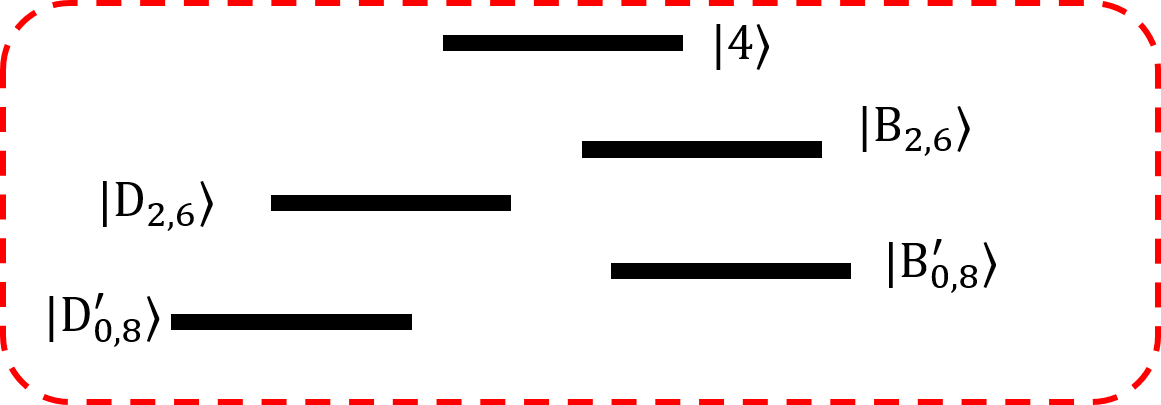
\includegraphics[width=10cm]{file/fig/effective_0and8/KPO_effective_0and8_5.png} \\
\caption{有効模型の概念図}
\label{fig:kpo_effective_0and8_5}
\end{figure}

上での摂動計算によって,摂動論により,補正された固有状態が次のように得られた:
\begin{align}
    \ket{B_{0,8}^{\prime}}
    &\equiv\ket{\varphi_{n,0}}
     = \frac{1}{\sqrt{2}}(\ket{0}+\ket{8}) + \delta_1\ket{B_{2,6}},\\[10pt]
     \delta_1 &\equiv \frac{p}{(\epsilon_0-\epsilon_{B_{2,6}})}\\[10pt]
    \ket{D_{0,8}^{\prime}}
    &\equiv\ket{\varphi_{n,8}}
     = \frac{1}{\sqrt{2}}(-\ket{0}+\ket{8}) + \delta_2\ket{D_{2,6}},\\[10pt]
     \delta_2 &\equiv \frac{p}{(\epsilon_0-\epsilon_{D_{2,6}})}
\end{align}
これで,すべての状態について,縮退が解け,縮退のない摂動論を用いて,有効模型のHamiltonianのエネルギー固有値,対応するエネルギー固有状態を求めることが可能となる.
\begin{figure}[h]
\centering
		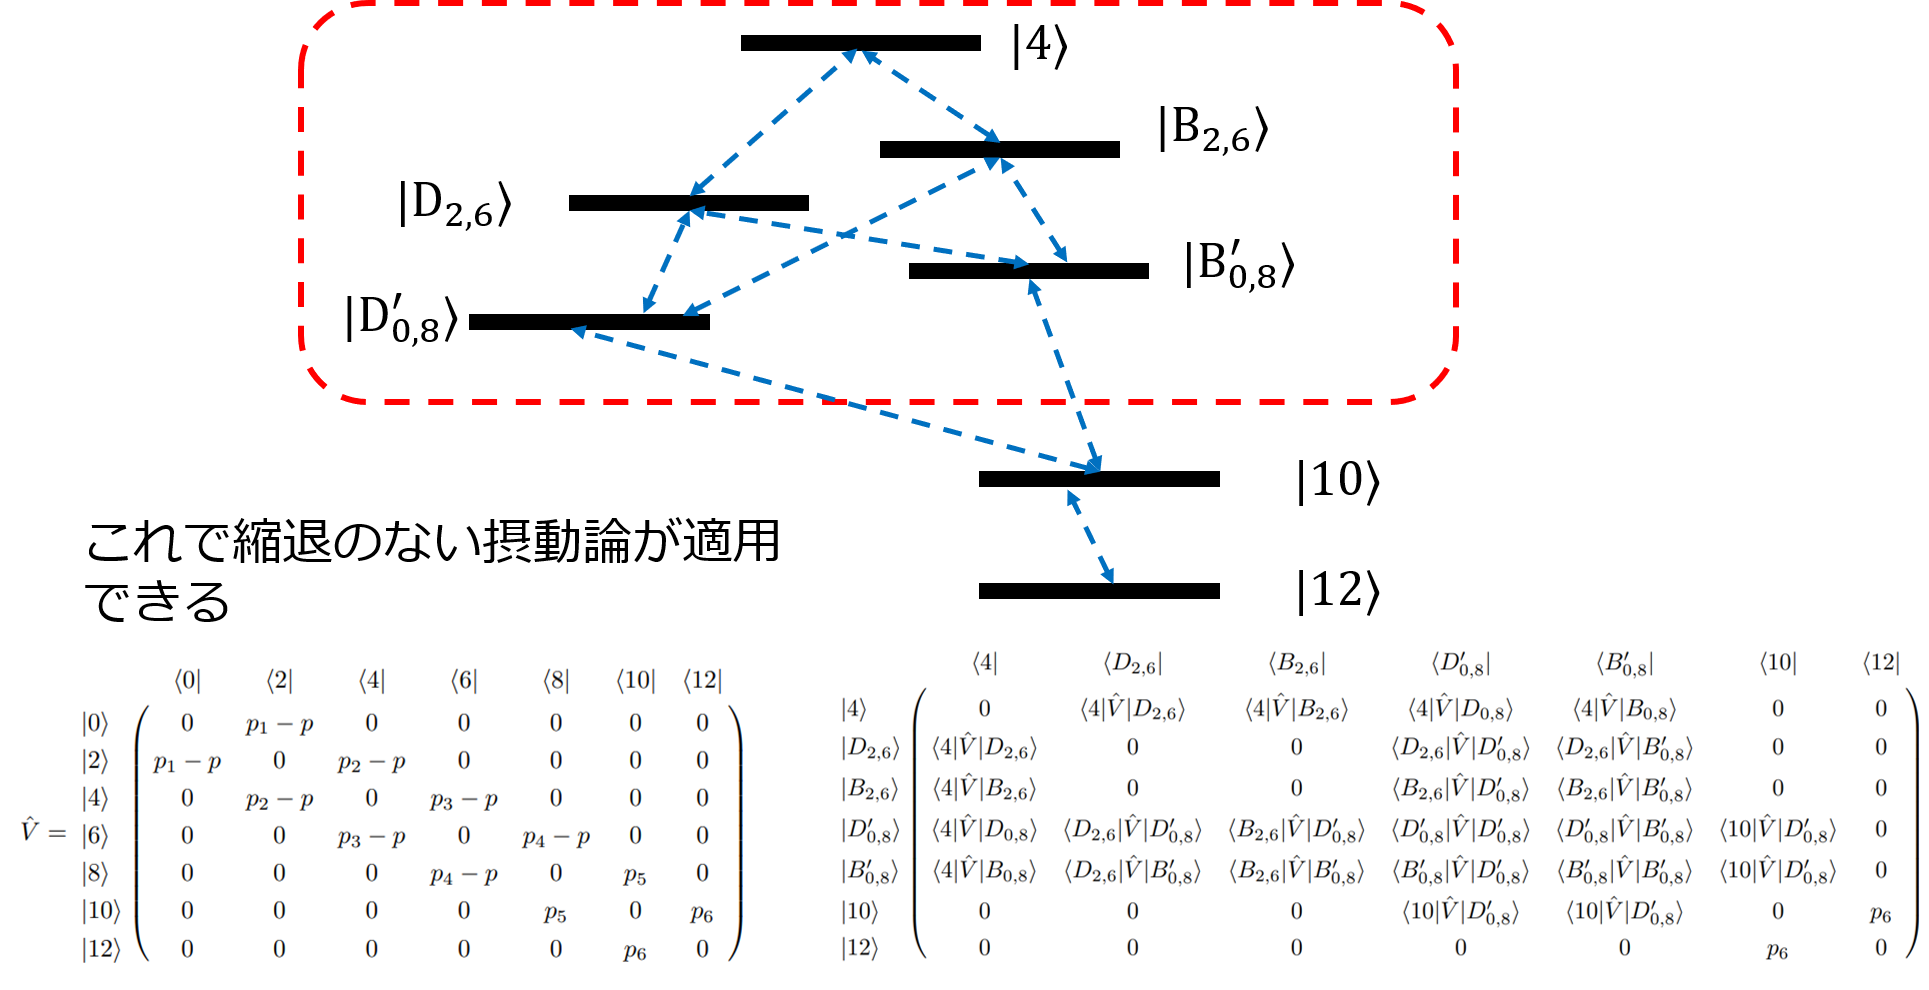
\includegraphics[width=10cm]{file/fig/effective_0and8/KPO_effective_0and8_6.png} \\
\caption{有効模型の概念図}
\label{fig:kpo_effective_0and8_6}
\end{figure}
まず,有効模型の摂動Hamiltonian
\begin{align}
  \hat{V}^{\rm{eff}}&=
   \bordermatrix{     
    & \bra{0} &  \bra{2} &  \bra{4}&  \bra{6}&  \bra{8} &\bra{10} &\bra{12}\cr
   \ket{0}&0&p_1-p&0&0&0&0&0\cr
  \ket{2}&p_1-p&0&p_2-p&0&0&0&0\cr
  \ket{4}&0&p_2-p&0&p_3-p&0&0&0\cr
  \ket{6}&0&0&p_3-p&0&p_4-p&0&0\cr
  \ket{8}&0&0&0&p_4-p&0&p_5&0\cr
  \ket{10}&0&0&0&0&p_5&0&p_6\cr
  \ket{12}&0&0&0&0&0&p_6&0\cr}
\end{align}
を基底$\{\bra{0},  \bra{2},  \bra{4}, \bra{6},  \bra{8}, \bra{10}, \bra{12}\}$で$\hat{V}^{\rm{eff}}$を表示すると,
\begin{align}
  \hat{V}^{\rm{eff}}&=
   \bordermatrix{     
    & \bra{4} &  \bra{D_{2,6}} &  \bra{B_{2,6}}&  \bra{D^\prime_{0,8}}&  \bra{B^\prime_{0,8}} &\bra{10} &\bra{12}\cr
   \ket{4}&0&\langle{4|\hat{V}|D_{2,6}}\rangle&\langle{4|\hat{V}|B_{2,6}}\rangle&\langle{4|\hat{V}|D_{0,8}}\rangle&\langle{4|\hat{V}|B_{0,8}}\rangle&0&0\cr
   %
  \ket{D_{2,6}}&\langle{4|\hat{V}|D_{2,6}}\rangle&0&0&\langle{D_{2,6}|\hat{V}|D^\prime_{0,8}}\rangle&\langle{D_{2,6}|\hat{V}|B^\prime_{0,8}}\rangle&0&0\cr
  %
  \ket{B_{2,6}}&\langle{4|\hat{V}|B_{2,6}}\rangle&0&0&\langle{B_{2,6}|\hat{V}|D^\prime_{0,8}}\rangle&\langle{B_{2,6}|\hat{V}|B^\prime_{0,8}}\rangle&0&0\cr
  %
  \ket{D^\prime_{0,8}}&\langle{4|\hat{V}|D_{0,8}}\rangle&\langle{D_{2,6}|\hat{V}|D^\prime_{0,8}}\rangle&\langle{B_{2,6}|\hat{V}|D^\prime_{0,8}}\rangle& \langle{D^\prime_{0,8}|\hat{V}|D^\prime_{0,8}}\rangle& \langle{D^\prime_{0,8}|\hat{V}|B^\prime_{0,8}}\rangle&\langle{10|\hat{V}|D^\prime_{0,8}}\rangle&0\cr
  %
  \ket{B^\prime_{0,8}}&\langle{4|\hat{V}|B_{0,8}}\rangle&\langle{D_{2,6}|\hat{V}|B^\prime_{0,8}}\rangle&\langle{B_{2,6}|\hat{V}|B^\prime_{0,8}}\rangle& \langle{B^\prime_{0,8}|\hat{V}|D^\prime_{0,8}}\rangle& \langle{B^\prime_{0,8}|\hat{V}|B^\prime_{0,8}}\rangle&\langle{10|\hat{V}|D^\prime_{0,8}}\rangle&0\cr
  %
  \ket{10}&0&0&0&\langle{10|\hat{V}|D^\prime_{0,8}}\rangle&\langle{10|\hat{V}|D^\prime_{0,8}}\rangle&0&p_6\cr
  %
  \ket{12}&0&0&0&0&0&p_6&0\cr}
\end{align}
となる.行列要素が,0となる場合だけ,あからさまに0と記述した.それ以外の,行列要素の具体的な値は,以下のように求まる:
\begin{align}
    \langle{4|\hat{V}|4}\rangle
    &=0\\[10pt]
    %
    \langle{4|\hat{V}|D_{2,6}}\rangle
    &=\langle{D_{2,6}|\hat{V}|4}\rangle
    =\frac{1}{\sqrt{2}}(-\braket{4|\hat{V}|2} + \braket{4|\hat{V}|6})
    =\frac{1}{\sqrt{2}}\Bigl\{
    -(p_2-p) + (p_3-p)
    \Bigr\}\\[10pt]
    %
    \langle{4|\hat{V}|B_{2,6}}\rangle
    &=\langle{B_{2,6}|\hat{V}|4}\rangle
    =\frac{1}{\sqrt{2}}(\braket{4|\hat{V}|2} + \braket{4|\hat{V}|6})
    =\frac{1}{\sqrt{2}}\Bigl\{
    (p_2-p) + (p_3-p)
    \Bigr\}\\[10pt]
    %
    \langle{4|\hat{V}|D_{0,8}}\rangle
    &=\langle{D_{0,8}|\hat{V}|4}\rangle
    =\frac{1}{\sqrt{2}}(-\braket{4|\hat{V}|0} + \braket{4|\hat{V}|8})
    +\delta_2\langle{4|\hat{V}|D_{2,6}}\rangle\nn[10pt]
    &=\frac{1}{\sqrt{2}}(0+0)
    +\frac{\delta_2}{\sqrt{2}}\Bigl\{
    -(p_2-p) + (p_3-p)
    \Bigr\}\\[10pt]
    %
   \langle{4|\hat{V}|B_{0,8}}\rangle
   &=\langle{B_{0,8}|\hat{V}|4}\rangle
   =\frac{1}{\sqrt{2}}(\braket{4|\hat{V}|0} + \braket{4|\hat{V}|8})
    +\delta_2\langle{4|\hat{V}|B_{2,6}}\rangle\nn[10pt]
    &=\frac{1}{\sqrt{2}}(0+0)
    +\frac{\delta_1}{\sqrt{2}}\Bigl\{
    (p_2-p) + (p_3-p)
    \Bigr\}\\[10pt]
\end{align}



\begin{align}
    %
    \langle{D_{2,6}|\hat{V}|D_{2,6}}\rangle
    &
    =\frac{1}{2}(-\braket{2|\hat{V}|6} - \braket{6|\hat{V}|2})
    =0\\[10pt]
    %
    \langle{D_{2,6}|\hat{V}|B_{2,6}}\rangle
    &=\langle{B_{2,6}|\hat{V}|D_{2,6}}\rangle
    =\frac{1}{2}(-\braket{2|\hat{V}|6} + \braket{6|\hat{V}|2})
    =0\\[10pt]
    %
    \langle{D_{2,6}|\hat{V}|D^\prime_{0,8}}\rangle
    &=\langle{D^\prime_{0,8}|\hat{V}|D_{2,6}}\rangle
    =\braket{D_{2,6}|\hat{V}|D_{0,8}} 
    +\delta_2\langle{D_{2,6}|\hat{V}|D_{2,6}}\rangle\nn[10pt]
    &=\frac{1}{2}(\braket{2|\hat{V}|0}+\braket{6|\hat{V}|8})
    +\delta_2\cdot0\nn[10pt]
    &=\frac{1}{2}\Bigl\{
    (p_1-p) + (p_4-p)
    \Bigr\}\\[10pt]
    %
   \langle{D_{2,6}|\hat{V}|B^\prime_{0,8}}\rangle
   &=\langle{B^\prime_{0,8}|\hat{V}|D_{2,6}}\rangle
    =\braket{D_{2,6}|\hat{V}|B_{0,8}} 
    +\delta_1\langle{D_{2,6}|\hat{V}|B_{2,6}}\rangle\nn[10pt]
    &=\frac{1}{2}(-\braket{2|\hat{V}|0}+\braket{6|\hat{V}|8})
    +\delta_1\cdot0\nn[10pt]
    &=\frac{1}{2}\Bigl\{
    -(p_1-p) + (p_4-p)
    \Bigr\}
\end{align}





\begin{align}
    %
    \langle{B_{2,6}|\hat{V}|B_{2,6}}\rangle
    &
    =\frac{1}{2}(\braket{2|\hat{V}|6} + \braket{6|\hat{V}|2})
    =0\\[10pt]
    %
    \langle{B_{2,6}|\hat{V}|D^\prime_{0,8}}\rangle
    &=\langle{D^\prime_{0,8}|\hat{V}|B_{2,6}}\rangle
    =\braket{B_{2,6}|\hat{V}|D_{0,8}} 
    +\delta_2\langle{B_{2,6}|\hat{V}|D_{2,6}}\rangle\nn[10pt]
    &=\frac{1}{2}(-\braket{2|\hat{V}|0}+\braket{6|\hat{V}|8})
    +\delta_2\cdot0\nn[10pt]
    &=\frac{1}{2}\Bigl\{
    -(p_1-p) + (p_4-p)
    \Bigr\}\\[10pt]
    %
   \langle{B_{2,6}|\hat{V}|B^\prime_{0,8}}\rangle
   &=\langle{B^\prime_{0,8}|\hat{V}|B_{2,6}}\rangle
    =\braket{B_{2,6}|\hat{V}|B_{0,8}} 
    +\delta_1\langle{B_{2,6}|\hat{V}|B_{2,6}}\rangle\nn[10pt]
    &=\frac{1}{2}(\braket{2|\hat{V}|0}+\braket{6|\hat{V}|8})
    +\delta_1\cdot0\nn[10pt]
    &=\frac{1}{2}\Bigl\{
    (p_1-p) + (p_4-p)
    \Bigr\}
\end{align}





a
\begin{align}
    \langle{D^\prime_{0,8}|\hat{V}|D^\prime_{0,8}}\rangle
    &=\Bigl(\bra{D_{2,6}} + \delta_2\bra{D_{0,8}}
    \Bigr)
    \hat{V}
    \Bigl(\ket{D_{2,6}} + \delta_2\ket{D_{0,8}}
    \Bigr)\nn[10pt]
    &=\langle{D_{0,8}|\hat{V}|D_{0,8}}\rangle
    +\delta_2^2\braket{D_{2,6}|\hat{V}|D_{2,6}} 
    +2\delta_2\langle{D_{2,6}|\hat{V}|D_{0,8}}\rangle\nn[10pt]
     &=2\delta_2\langle{D_{2,6}|\hat{V}|D_{0,8}}\rangle\nn[10pt]
    &=2\delta_2\frac{1}{2}(\braket{2|\hat{V}|0}+\braket{6|\hat{V}|8})
    \nn[10pt]
    &=\delta_2\Bigl\{
    (p_1-p) + (p_4-p)
    \Bigr\}\\[10pt]
    %
    %
   \langle{D^\prime_{0,8}|\hat{V}|B^\prime_{0,8}}\rangle
   &=\Bigl(\bra{D_{2,6}} + \delta_2\bra{D_{0,8}}
    \Bigr)
    \hat{V}
    \Bigl(\ket{B_{2,6}} + \delta_1\ket{B_{0,8}}
    \Bigr)\nn[10pt]
    &=\langle{D_{0,8}|\hat{V}|B_{0,8}}\rangle
    +\delta_1\delta_2\braket{D_{2,6}|\hat{V}|B_{2,6}} 
    +(\delta_1+\delta_2)\langle{D_{2,6}|\hat{V}|B_{0,8}}\rangle\nn[10pt]
     &=(\delta_1+\delta_2)\langle{D_{2,6}|\hat{V}|B_{0,8}}\rangle\nn[10pt]
    &=(\delta_1+\delta_2)\frac{1}{2}(-\braket{2|\hat{V}|0}+\braket{6|\hat{V}|8})
    \nn[10pt]
    &=\frac{\delta_1+\delta_2}{2}\Bigl\{
    -(p_1-p) + (p_4-p)
    \Bigr\}
\end{align}



a
\begin{align}
    \langle{B^\prime_{0,8}|\hat{V}|D^\prime_{0,8}}\rangle
    &=\langle{D^\prime_{0,8}|\hat{V}|B^\prime_{0,8}}\rangle\nn[10pt]
    %
   \langle{B^\prime_{0,8}|\hat{V}|B^\prime_{0,8}}\rangle
   &=\Bigl(\bra{B_{2,6}} + \delta_1\bra{D_{0,8}}
    \Bigr)
    \hat{V}
    \Bigl(\ket{B_{2,6}} + \delta_1\ket{B_{0,8}}
    \Bigr)\nn[10pt]
    &=\langle{B_{0,8}|\hat{V}|B_{0,8}}\rangle
    +\delta_1^2\braket{B_{2,6}|\hat{V}|B_{2,6}} 
    +2\delta_1\langle{B_{2,6}|\hat{V}|B_{0,8}}\rangle\nn[10pt]
     &=2\delta_1\langle{B_{2,6}|\hat{V}|B_{0,8}}\rangle\nn[10pt]
    &=2\delta_1\frac{1}{2}(\braket{2|\hat{V}|0}+\braket{6|\hat{V}|8})
    \nn[10pt]
    &=\delta_1\Bigl\{
    (p_1-p) + (p_4-p)
    \Bigr\}
\end{align}




b
\begin{align}
    \langle{10|\hat{V}|D^\prime_{0,8}}\rangle
    &=\langle{10|\hat{V}|B^\prime_{0,8}}\rangle\nn[10pt]
    %
   &=\langle{10|\hat{V}|D_{0,8}}\rangle
    +\delta_2\braket{10|\hat{V}|D_{2,6}}\nn[10pt]
     &=\frac{1}{\sqrt{2}}\langle{10|\hat{V}|8}\rangle\nn[10pt]
    &=\frac{1}{\sqrt{2}}p_5
\end{align}


次に縮退のない摂動論を実行するため,計算しやすいように,固有状態の第ゼロ近似それぞれに,次のようにラベルを付ける:
\begin{align}
    \ket{\varphi_{0}^{(0)}}&\equiv\ket{4}\\[5pt]
    \ket{\varphi_{1}^{(0)}}&\equiv\ket{D_{2,6}}\\[5pt]
    \ket{\varphi_{2}^{(0)}}&\equiv\ket{B_{2,6}}\\[5pt]
    \ket{\varphi_{3}^{(0)}}&\equiv\ket{D^\prime_{0,8}}\\[5pt]
    \ket{\varphi_{4}^{(0)}}&\equiv\ket{B^\prime_{0,8}}\\[5pt]
    \ket{\varphi_{5}^{(0)}}&\equiv\ket{10}\\[5pt]
    \ket{\varphi_{6}^{(0)}}&\equiv\ket{12}
\end{align}


固有状態の2次の近似の公式は
\begin{align}
\ket{\varphi_{n}}&\simeq\ket{\varphi_{n}^{(0)}}+\lambda\ket{\varphi_{n}^{(1)}}+\lambda^2\ket{\varphi_{n}^{(2)}}\notag\\[10pt]
&=\ket{\varphi_{n}^{(0)}}
+
\displaystyle\sum_{\substack{m=1 \\ m\neq n}}^\infty
 \frac{\braket{\varphi_{m
 }^{(0)}|\lambda\hat{V}|\varphi_{n}^{(0)}}}{(\epsilon_{n}-\epsilon_{m})}
\ket{\varphi_{m}^{(0)}}\notag\\[10pt]
&+\lambda^2
\displaystyle\sum_{\substack{m=1 \\ m\neq n}}^\infty
 \left[\left(
\displaystyle\sum_{\substack{k=1 \\ k\neq n}}^\infty
 \frac{
  \bra{\varphi_{m}^{(0)}}\hat{V}\ket{\varphi_{k}^{(0)}}
 \braket{\varphi_{k}^{(0)}|\hat{V}|\varphi_{n}^{(0)}}
 }{(\epsilon_{n}-\epsilon_{k})(\epsilon_{n}-\epsilon_{m})}
    \right)
  -
   \frac{
\braket{\varphi_{n}^{(0)}|\hat{V}|\varphi_{n}^{(0)}}\braket{\varphi_{m}^{(0)}|\hat{V}|\varphi_{n}^{(0)}}}{(\epsilon_{n}-\epsilon_{m})^2}
  \right]
\ket{\varphi_{m}^{(0)}}
\end{align}
で与えられる.これに,代入し,補正項を求めていくことにする:

$ith : 8, 0 : [[0.70710437+0.j]], 2 : [[0.00151543+0.j]], 4 : [[5.58643597e-05+0.j]], 6 : [[0.00801705+0.j]],  8 : [[0.70703581+0.j]], 10 : [[-0.00609805+0.j]],  12 : [[2.65387791e-05+0.j]]$



\subsection*{1次の摂動}
\begin{align}
    \ket{\varphi_{4}^{(1)}}
    &=
    \displaystyle\sum_{\substack{m=1 \\ m\neq 4}}^\infty
     \frac{\braket{\varphi_{m
     }^{(0)}|\hat{V}|\varphi_{4}^{(0)}}}{(\epsilon_{4}-\epsilon_{m})}\ket{\varphi_{m}^{(0)}}\nn[10pt]
     %%%%%%%%%%%%%%%%%%%%%
     %%%%%%%%%%%%%%%%%%%%%
     &=\frac{\braket{\varphi_{0
     }^{(0)}|\hat{V}|\varphi_{4}^{(0)}}}{(\epsilon_{4}-\epsilon_{0})}\ket{\varphi_{0}^{(0)}}
     +
     \frac{\braket{\varphi_{1
     }^{(0)}|\hat{V}|\varphi_{4}^{(0)}}}{(\epsilon_{4}-\epsilon_{1})}\ket{\varphi_{1}^{(0)}}
     +
     \frac{\braket{\varphi_{2
     }^{(0)}|\hat{V}|\varphi_{4}^{(0)}}}{(\epsilon_{4}-\epsilon_{2})}\ket{\varphi_{2}^{(0)}}
     \nn[10pt]
     &+
     \frac{\braket{\varphi_{3
     }^{(0)}|\hat{V}|\varphi_{4}^{(0)}}}{(\epsilon_{4}-\epsilon_{3})}\ket{\varphi_{3}^{(0)}}
     +
     \frac{\braket{\varphi_{5
     }^{(0)}|\hat{V}|\varphi_{4}^{(0)}}}{(\epsilon_{4}-\epsilon_{5})}\ket{\varphi_{5}^{(0)}}
     +
     \frac{\braket{\varphi_{6
     }^{(0)}|\hat{V}|\varphi_{4}^{(0)}}}{(\epsilon_{4}-\epsilon_{6})}\ket{\varphi_{6}^{(0)}}
\end{align}


\begin{equation}
    \ket{\Psi_{4,i}^{(1)}}
    \equiv 
    \frac{\braket{\varphi_{i
     }^{(0)}|\hat{V}|\varphi_{4}^{(0)}}}{(\epsilon_{4}-\epsilon_{i})}\ket{\varphi_{i}^{(0)}}
\end{equation}




\begin{align}
    \ket{\Psi_{4,0}^{(1)}}
     &=\frac{\braket{\varphi_{0
     }^{(0)}|\hat{V}|\varphi_{4}^{(0)}}}{(\epsilon_{4}-\epsilon_{0})}\ket{\varphi_{0}^{(0)}}
     =\frac{\braket{4|\hat{V}|B_{0,8}^{\prime}}}{(E_{B_{0,8}^{\prime}}-E_4)}\ket{4}
     \nn[10pt]
     &=
     \frac{1}{(E_{B_{0,8}^{\prime}}-E_4)}
     \frac{\delta_1}{\sqrt{2}}(p_2+p_3-2p)
     \ket{4}
     =
     \frac{p(p_2+p_3-2p)}{\sqrt{2}(E_{B_{0,8}^{\prime}}-E_4)(E_0-E_{B_{2,6}})}
     \ket{4}
\end{align}
 %%%%%%%%%%%%%%%%%%%
%%%%%%%%%%%%%%%%%%%
\begin{align}
     \ket{\Psi_{4,1}^{(1)}}
     &=
     \frac{\braket{\varphi_{1
     }^{(0)}|\hat{V}|\varphi_{4}^{(0)}}}{(\epsilon_{4}-\epsilon_{1})}\ket{\varphi_{1}^{(0)}}
      =\frac{\braket{D_{2,6}|\hat{V}|B_{0,8}^{\prime}}}{(E_{B_{0,8}^{\prime}}-E_{D_{2,6}})}\ket{D_{2,6}}\nn[10pt]
      &=\frac{1}{(E_{B_{0,8}^{\prime}}-E_{D_{2,6}})}
      \frac{1}{2}(-p_1+p_4)
      \ket{D_{2,6}}
      =\frac{-p_1+p_4}{2(E_{B_{0,8}^{\prime}}-E_{D_{2,6}})}
      \ket{D_{2,6}}
\end{align}
%%%%%%%%%%%%%%%%%%%
%%%%%%%%%%%%%%%%%%%
\begin{align}
     \ket{\Psi_{4,2}^{(1)}}
     &=
     \frac{\braket{\varphi_{2
     }^{(0)}|\hat{V}|\varphi_{4}^{(0)}}}{(\epsilon_{4}-\epsilon_{2})}\ket{\varphi_{2}^{(0)}}
      =\frac{\braket{B_{2,6}|\hat{V}|B_{0,8}^{\prime}}}{(E_{B_{0,8}^{\prime}}-E_{B_{2,6}})}\ket{B_{2,6}}\nn[10pt]
      &=\frac{1}{(E_{B_{0,8}^{\prime}}-E_{B_{2,6}})}
      \frac{1}{2}(p_1+p_4-2p)
      \ket{B_{2,6}}
      =\frac{(p_1+p_4-2p)}{2(E_{B_{0,8}^{\prime}}-E_{B_{2,6}})}
      \ket{B_{2,6}}
\end{align}
     %%%%%%%%%%%%%%%%%%%
    %%%%%%%%%%%%%%%%%%%
\begin{align}
     \ket{\Psi_{4,3}^{(1)}}
     &=
     \frac{\braket{\varphi_{3
     }^{(0)}|\hat{V}|\varphi_{4}^{(0)}}}{(\epsilon_{4}-\epsilon_{3})}\ket{\varphi_{3}^{(0)}}
      =\frac{\braket{D_{0,8}^{\prime}|\hat{V}|B_{0,8}^{\prime}}}{(E_{B_{0,8}^{\prime}}-E_{D_{0,8}^{\prime}})}\ket{D_{0,8}^{\prime}}\nn[10pt]
      &=\frac{1}{(E_{B_{0,8}^{\prime}}-E_{D_{0,8}^{\prime}})}
      \frac{\delta_1+\delta_2}{2}(-p_1+p_4)\ket{D_{0,8}^{\prime}}
      =\frac{(\delta_1+\delta_2)(-p_1+p_4)}
      {2(E_{B_{0,8}^{\prime}}-E_{D_{0,8}^{\prime}})}
      \ket{D_{0,8}^{\prime}}
\end{align}
 %%%%%%%%%%%%%%%%%%%
%%%%%%%%%%%%%%%%%%%
\begin{align}
     \ket{\Psi_{4,5}^{(1)}}
     &=
     \frac{\braket{\varphi_{5
     }^{(0)}|\hat{V}|\varphi_{4}^{(0)}}}{(\epsilon_{4}-\epsilon_{5})}\ket{\varphi_{5}^{(0)}}
      =\frac{\braket{10|\hat{V}|B_{0,8}^{\prime}}}{(E_{B_{0,8}^{\prime}}-E_{10})}\ket{10}
      =\frac{p_5}{\sqrt{2}(E_{B_{0,8}^{\prime}}-E_{10})}\ket{10}
\end{align}
\begin{align}
     %%%%%%%%%%%%%%%%%%%
    %%%%%%%%%%%%%%%%%%%
     \ket{\Psi_{4,6}^{(1)}}
     &=
     \frac{\braket{\varphi_{6
     }^{(0)}|\hat{V}|\varphi_{4}^{(0)}}}{(\epsilon_{4}-\epsilon_{6})}\ket{\varphi_{6}^{(0)}}
      =\frac{\braket{12|\hat{V}|B_{0,8}^{\prime}}}{(E_{B_{0,8}^{\prime}}-E_{12})}\ket{12}=0\cdot\ket{12}
\end{align}
ここで,
$p_1=\sqrt{2\cdot1}p$, $p_2=\sqrt{4\cdot3}p$, $p_3=\sqrt{6\cdot5}p$, $p_4=\sqrt{8\cdot7}p$, $p_5=\sqrt{10\cdot9}p$, $p_6=\sqrt{12\cdot11}p$
である.

\subsection*{2次の摂動}
\begin{align}
\ket{\varphi_{n}^{(2)}}
&=
\displaystyle\sum_{\substack{m=1 \\ m\neq n}}^\infty
 \left[\left(
\displaystyle\sum_{\substack{k=1 \\ k\neq n}}^\infty
 \frac{
  \bra{\varphi_{m}^{(0)}}\hat{V}\ket{\varphi_{k}^{(0)}}
 \braket{\varphi_{k}^{(0)}|\hat{V}|\varphi_{n}^{(0)}}
 }{(\epsilon_{n}-\epsilon_{k})(\epsilon_{n}-\epsilon_{m})}
    \right)
  -
   \frac{
\braket{\varphi_{n}^{(0)}|\hat{V}|\varphi_{n}^{(0)}}\braket{\varphi_{m}^{(0)}|\hat{V}|\varphi_{n}^{(0)}}}{(\epsilon_{n}-\epsilon_{m})^2}
  \right]
\ket{\varphi_{m}^{(0)}}
\end{align}




\begin{equation}
    \ket{\Psi_{4,i}^{(2)}}
    \equiv 
     \left[\left(
    \displaystyle\sum_{\substack{k=1 \\ k\neq 4}}^\infty
     \frac{
      \bra{\varphi_{i}^{(0)}}\hat{V}\ket{\varphi_{k}^{(0)}}
     \braket{\varphi_{k}^{(0)}|\hat{V}|\varphi_{4}^{(0)}}
     }{(\epsilon_{4}-\epsilon_{k})(\epsilon_{4}-\epsilon_{i})}
        \right)
      -
       \frac{
    \braket{\varphi_{4}^{(0)}|\hat{V}|\varphi_{4}^{(0)}}\braket{\varphi_{i}^{(0)}|\hat{V}|\varphi_{4}^{(0)}}}{(\epsilon_{4}-\epsilon_{i})^2}
      \right]
    \ket{\varphi_{i}^{(0)}}
\end{equation}




\begin{align}
    \ket{\Psi_{4,0}^{(2)}}
     &=\frac{\braket{\varphi_{0
     }^{(0)}|\hat{V}|\varphi_{4}^{(0)}}}{(\epsilon_{4}-\epsilon_{0})}\ket{\varphi_{0}^{(0)}}
     =\frac{\braket{4|\hat{V}|B_{0,8}^{\prime}}}{(E_{B_{0,8}^{\prime}}-E_4)}\ket{4}
     \nn[10pt]
     &=
     \frac{1}{(E_{B_{0,8}^{\prime}}-E_4)}
     \frac{\delta_1}{\sqrt{2}}(p_2+p_3-2p)
     \ket{4}
     =
     \frac{p(p_2+p_3-2p)}{\sqrt{2}(E_{B_{0,8}^{\prime}}-E_4)(E_0-E_{B_{2,6}})}
     \ket{4}
\end{align}
 %%%%%%%%%%%%%%%%%%%
%%%%%%%%%%%%%%%%%%%
\begin{align}
     \ket{\Psi_{4,1}^{(1)}}
     &=
     \frac{\braket{\varphi_{1
     }^{(0)}|\hat{V}|\varphi_{4}^{(0)}}}{(\epsilon_{4}-\epsilon_{1})}\ket{\varphi_{1}^{(0)}}
      =\frac{\braket{D_{2,6}|\hat{V}|B_{0,8}^{\prime}}}{(E_{B_{0,8}^{\prime}}-E_{D_{2,6}})}\ket{D_{2,6}}\nn[10pt]
      &=\frac{1}{(E_{B_{0,8}^{\prime}}-E_{D_{2,6}})}
      \frac{1}{2}(-p_1+p_4)
      \ket{D_{2,6}}
      =\frac{-p_1+p_4}{2(E_{B_{0,8}^{\prime}}-E_{D_{2,6}})}
      \ket{D_{2,6}}
\end{align}
%%%%%%%%%%%%%%%%%%%
%%%%%%%%%%%%%%%%%%%
\begin{align}
     \ket{\Psi_{4,2}^{(1)}}
     &=
     \frac{\braket{\varphi_{2
     }^{(0)}|\hat{V}|\varphi_{4}^{(0)}}}{(\epsilon_{4}-\epsilon_{2})}\ket{\varphi_{2}^{(0)}}
      =\frac{\braket{B_{2,6}|\hat{V}|B_{0,8}^{\prime}}}{(E_{B_{0,8}^{\prime}}-E_{B_{2,6}})}\ket{B_{2,6}}\nn[10pt]
      &=\frac{1}{(E_{B_{0,8}^{\prime}}-E_{B_{2,6}})}
      \frac{1}{2}(p_1+p_4-2p)
      \ket{B_{2,6}}
      =\frac{(p_1+p_4-2p)}{2(E_{B_{0,8}^{\prime}}-E_{B_{2,6}})}
      \ket{B_{2,6}}
\end{align}
     %%%%%%%%%%%%%%%%%%%
    %%%%%%%%%%%%%%%%%%%
\begin{align}
     \ket{\Psi_{4,3}^{(1)}}
     &=
     \frac{\braket{\varphi_{3
     }^{(0)}|\hat{V}|\varphi_{4}^{(0)}}}{(\epsilon_{4}-\epsilon_{3})}\ket{\varphi_{3}^{(0)}}
      =\frac{\braket{D_{0,8}^{\prime}|\hat{V}|B_{0,8}^{\prime}}}{(E_{B_{0,8}^{\prime}}-E_{D_{0,8}^{\prime}})}\ket{D_{0,8}^{\prime}}\nn[10pt]
      &=\frac{1}{(E_{B_{0,8}^{\prime}}-E_{D_{0,8}^{\prime}})}
      \frac{\delta_1+\delta_2}{2}(-p_1+p_4)\ket{D_{0,8}^{\prime}}
      =\frac{(\delta_1+\delta_2)(-p_1+p_4)}
      {2(E_{B_{0,8}^{\prime}}-E_{D_{0,8}^{\prime}})}
      \ket{D_{0,8}^{\prime}}
\end{align}
 %%%%%%%%%%%%%%%%%%%
%%%%%%%%%%%%%%%%%%%
\begin{align}
     \ket{\Psi_{4,5}^{(1)}}
     &=
     \frac{\braket{\varphi_{5
     }^{(0)}|\hat{V}|\varphi_{4}^{(0)}}}{(\epsilon_{4}-\epsilon_{5})}\ket{\varphi_{5}^{(0)}}
      =\frac{\braket{10|\hat{V}|B_{0,8}^{\prime}}}{(E_{B_{0,8}^{\prime}}-E_{10})}\ket{10}
      =\frac{p_5}{\sqrt{2}(E_{B_{0,8}^{\prime}}-E_{10})}\ket{10}
\end{align}
\begin{align}
     %%%%%%%%%%%%%%%%%%%
    %%%%%%%%%%%%%%%%%%%
     \ket{\Psi_{4,6}^{(1)}}
     &=
     \frac{\braket{\varphi_{6
     }^{(0)}|\hat{V}|\varphi_{4}^{(0)}}}{(\epsilon_{4}-\epsilon_{6})}\ket{\varphi_{6}^{(0)}}
      =\frac{\braket{12|\hat{V}|B_{0,8}^{\prime}}}{(E_{B_{0,8}^{\prime}}-E_{12})}\ket{12}=0\cdot\ket{12}
\end{align}


%%%%%%%%%%%%%%%%%%%%%%%%%%%%%%%%%%%%%
%%%%%%%%%%%%%%%%%%%%%%%%%%%%%%%%%%%%%
%%%%%%%%%%%%%%%%%%%%%%%%%%%%%%%%%%%%%
%%%%%%%%%%%%%%%%%%%%%%%%%%%%%%%%%%%%%
%%%%%%%%%%%%%%%%%%%%%%%%%%%%%%%%%%%%%
%%%%%%%%%%%%%%%%%%%%%%%%%%%%%%%%%%%%%
% \subsection{$n=0$と$n=12$が縮退している場合}
% まず,$n=0$と$n=12$が縮退している場合を考えよう.この場合のHamiltonianは以下のように書ける:
% \begin{align}
%      \hat{H}_{\rm{KPO}}&=
%    \bordermatrix{     
%     & \bra{0} &  \bra{2} &  \bra{4}&  \bra{6}&  \bra{8} &\bra{10} &\bra{12}\cr
%    \ket{0}&E_0&\sqrt{2\cdot1}p&0&0&0&0&0\cr
%   \ket{2}&\sqrt{2\cdot1}p&E_2&\sqrt{4\cdot3}p&0&0&0&0\cr
%   \ket{4}&0&\sqrt{4\cdot3}p&E_4&\sqrt{6\cdot5}p&0&0&0\cr
%   \ket{6}&0&0&\sqrt{6\cdot5}p&E_6&\sqrt{8\cdot7}p&0&0\cr
%   \ket{8}&0&0&0&\sqrt{8\cdot7}p&E_8&\sqrt{10\cdot9}p&0\cr
%   \ket{10}&0&0&0&0&\sqrt{10\cdot9}p&E_{10}&\sqrt{12\cdot11}p\cr
%   \ket{12}&0&0&0&0&0&\sqrt{12\cdot11}p&E_{12}\cr
%             }\\[10pt]
%     &=
%    \bordermatrix{     
%     & \bra{0} &  \bra{2} &  \bra{4}&  \bra{6}&  \bra{8} &\bra{10} &\bra{12}\cr
%    \ket{0}&0&\sqrt{2\cdot1}p&0&0&0&0&0\cr
%   \ket{2}&\sqrt{2\cdot1}p&\Delta_1&\sqrt{4\cdot3}p&0&0&0&0\cr
%   \ket{4}&0&\sqrt{4\cdot3}p&\Delta_2&\sqrt{6\cdot5}p&0&0&0\cr
%   \ket{6}&0&0&\sqrt{6\cdot5}p&\Delta_3&\sqrt{8\cdot7}p&0&0\cr
%   \ket{8}&0&0&0&\sqrt{8\cdot7}p&\Delta_2&\sqrt{10\cdot9}p&0\cr
%   \ket{10}&0&0&0&0&\sqrt{10\cdot9}p&\Delta_1&\sqrt{12\cdot11}p\cr
%   \ket{12}&0&0&0&0&0&\sqrt{12\cdot11}p&0\cr
%             }
% \end{align}
% ここで,$E_0=E_12=0$, $E_2=E_{10}=\Delta_1$, $E_4=E_{8}=\Delta_2$, $E_=\Delta_3$である.





% \begin{align}
%     \hat{H}_0 &= E_{2}\ket{2}\bra{2} + E_{10} \ket{10}\bra{10} + E_{D_{4,8}} \ket{D_{4,8}}\bra{D_{4,8}}+ E_{B_{4,8}} \ket{B_{4,8}}\bra{B_{4,8}}\\[10pt]
%     \hat{V}&= \sqrt{4\cdot3}p\ket{2}\bra{4} + \sqrt{10\cdot9}p\ket{10}\bra{8} + {\rm{h.c.}}
% \end{align}


% \begin{align}
%      \hat{H}_{\rm{KPO}}
%     &=
%    \bordermatrix{     
%     & \bra{2} &  \bra{2} &  \bra{6}&  \bra{8}\cr
%    \ket{0}&0&\sqrt{2\cdot1}p&0&0\cr
%   \ket{2}&\sqrt{2\cdot1}p&\Delta_1&0&0\cr
%   \ket{6}&0&0&\Delta_1&\sqrt{8\cdot7}p\cr
%   \ket{8}&0&0&\sqrt{8\cdot7}p&0\cr
%             }
% \end{align}
% 次の状態を定義する:
% \begin{align}
%     \ket{D_{4,8}} &= \frac{1}{\sqrt{2}}(-\ket{4}+\ket{8})\\[10pt]
%     \ket{B_{4,8}} &= \frac{1}{\sqrt{2}}(\ket{4}+\ket{8})
% \end{align}
% 摂動Hamiltonianを基底$\{\ket{2},\ket{10},\ket{D_{4,8}},\ket{B_{4,8}}\}$で展開する:
% \begin{align}
%      \hat{V}
%     &=
%    \bordermatrix{     
%     & \bra{2} &  \bra{10} &  \bra{D_{4,8}}&  \bra{B_{4,8}}\cr
%    \ket{2}&\langle{2|\hat{V}|2}\rangle&\langle{2|\hat{V}|10}\rangle&\langle{2|\hat{V}|D_{4,8}}\rangle
%    &\langle{2|\hat{V}|B_{4,8}}\rangle\cr
%   \ket{10}&\langle{10|\hat{V}|2}\rangle&\langle{10|\hat{V}|10}\rangle&\langle{10|\hat{V}|D_{4,8}}\rangle
%    &\langle{10|\hat{V}|B_{4,8}}\rangle\cr
%   \ket{D_{4,8}}&\langle{D_{4,8}|\hat{V}|2}\rangle&\langle{D_{4,8}|\hat{V}|10}\rangle&\langle{D_{4,8}|\hat{V}|D_{4,8}}\rangle
%    &\langle{D_{4,8}|\hat{V}|B_{4,8}}\rangle\cr
%   \ket{B_{4,8}}&\langle{B_{4,8}|\hat{V}|2}\rangle&\langle{B_{4,8}|\hat{V}|10}\rangle&\langle{B_{4,8}|\hat{V}|D_{4,8}}\rangle
%    &\langle{B_{4,8}|\hat{V}|B_{4,8}}\rangle\cr
%     }\\[10pt]
%     &=
%    \bordermatrix{     
%    & \bra{2} &  \bra{10} &  \bra{D_{4,8}}&  \bra{B_{4,8}}\cr
%    \ket{2}&0&0&-\sqrt{4\cdot3}p/\sqrt{2}&\sqrt{4\cdot3}p/\sqrt{2}\cr
%   \ket{10}&0&0&\sqrt{10\cdot9}p/\sqrt{2}&\sqrt{10\cdot9}p/\sqrt{2}\cr
%   \ket{D_{4,8}}&-\sqrt{4\cdot3}p/\sqrt{2}&\sqrt{4\cdot3}p/\sqrt{2}&0&0\cr
%   \ket{B_{4,8}}&\sqrt{10\cdot9}p/\sqrt{2}&\sqrt{10\cdot9}p/\sqrt{2}&0&0&\cr
%             }
% \end{align}

% \begin{align}
%     \langle{2|\hat{V}|D_{4,8}}\rangle&=\langle{D_{4,8}|\hat{V}|2}\rangle
%     =-\sqrt{4\cdot3}p/\sqrt{2}\\[10pt]
%     \langle{2|\hat{V}|B_{4,8}}\rangle&=\langle{B_{4,8}|\hat{V}|2}\rangle
%     =\sqrt{4\cdot3}p/\sqrt{2}\\[10pt]
%     \langle{10|\hat{V}|D_{4,8}}\rangle&=\langle{D_{4,8}|\hat{V}|10}\rangle
%     =\sqrt{10\cdot9}p/\sqrt{2}\\[10pt]
%    \langle{10|\hat{V}|B_{4,8}}\rangle&=\langle{B_{4,8}|\hat{V}|10}\rangle
%    =\sqrt{10\cdot9}p/\sqrt{2}
% \end{align}


